
% Default to the notebook output style

    


% Inherit from the specified cell style.




    
\documentclass[11pt]{article}

    
    
    \usepackage[T1]{fontenc}
    % Nicer default font (+ math font) than Computer Modern for most use cases
    \usepackage{mathpazo}

    % Basic figure setup, for now with no caption control since it's done
    % automatically by Pandoc (which extracts ![](path) syntax from Markdown).
    \usepackage{graphicx}
    % We will generate all images so they have a width \maxwidth. This means
    % that they will get their normal width if they fit onto the page, but
    % are scaled down if they would overflow the margins.
    \makeatletter
    \def\maxwidth{\ifdim\Gin@nat@width>\linewidth\linewidth
    \else\Gin@nat@width\fi}
    \makeatother
    \let\Oldincludegraphics\includegraphics
    % Set max figure width to be 80% of text width, for now hardcoded.
    \renewcommand{\includegraphics}[1]{\Oldincludegraphics[width=.8\maxwidth]{#1}}
    % Ensure that by default, figures have no caption (until we provide a
    % proper Figure object with a Caption API and a way to capture that
    % in the conversion process - todo).
    \usepackage{caption}
    \DeclareCaptionLabelFormat{nolabel}{}
    \captionsetup{labelformat=nolabel}

    \usepackage{adjustbox} % Used to constrain images to a maximum size 
    \usepackage{xcolor} % Allow colors to be defined
    \usepackage{enumerate} % Needed for markdown enumerations to work
    \usepackage{geometry} % Used to adjust the document margins
    \usepackage{amsmath} % Equations
    \usepackage{amssymb} % Equations
    \usepackage{textcomp} % defines textquotesingle
    % Hack from http://tex.stackexchange.com/a/47451/13684:
    \AtBeginDocument{%
        \def\PYZsq{\textquotesingle}% Upright quotes in Pygmentized code
    }
    \usepackage{upquote} % Upright quotes for verbatim code
    \usepackage{eurosym} % defines \euro
    \usepackage[mathletters]{ucs} % Extended unicode (utf-8) support
    \usepackage[utf8x]{inputenc} % Allow utf-8 characters in the tex document
    \usepackage{fancyvrb} % verbatim replacement that allows latex
    \usepackage{grffile} % extends the file name processing of package graphics 
                         % to support a larger range 
    % The hyperref package gives us a pdf with properly built
    % internal navigation ('pdf bookmarks' for the table of contents,
    % internal cross-reference links, web links for URLs, etc.)
    \usepackage{hyperref}
    \usepackage{longtable} % longtable support required by pandoc >1.10
    \usepackage{booktabs}  % table support for pandoc > 1.12.2
    \usepackage[inline]{enumitem} % IRkernel/repr support (it uses the enumerate* environment)
    \usepackage[normalem]{ulem} % ulem is needed to support strikethroughs (\sout)
                                % normalem makes italics be italics, not underlines
    

    
    
    % Colors for the hyperref package
    \definecolor{urlcolor}{rgb}{0,.145,.698}
    \definecolor{linkcolor}{rgb}{.71,0.21,0.01}
    \definecolor{citecolor}{rgb}{.12,.54,.11}

    % ANSI colors
    \definecolor{ansi-black}{HTML}{3E424D}
    \definecolor{ansi-black-intense}{HTML}{282C36}
    \definecolor{ansi-red}{HTML}{E75C58}
    \definecolor{ansi-red-intense}{HTML}{B22B31}
    \definecolor{ansi-green}{HTML}{00A250}
    \definecolor{ansi-green-intense}{HTML}{007427}
    \definecolor{ansi-yellow}{HTML}{DDB62B}
    \definecolor{ansi-yellow-intense}{HTML}{B27D12}
    \definecolor{ansi-blue}{HTML}{208FFB}
    \definecolor{ansi-blue-intense}{HTML}{0065CA}
    \definecolor{ansi-magenta}{HTML}{D160C4}
    \definecolor{ansi-magenta-intense}{HTML}{A03196}
    \definecolor{ansi-cyan}{HTML}{60C6C8}
    \definecolor{ansi-cyan-intense}{HTML}{258F8F}
    \definecolor{ansi-white}{HTML}{C5C1B4}
    \definecolor{ansi-white-intense}{HTML}{A1A6B2}

    % commands and environments needed by pandoc snippets
    % extracted from the output of `pandoc -s`
    \providecommand{\tightlist}{%
      \setlength{\itemsep}{0pt}\setlength{\parskip}{0pt}}
    \DefineVerbatimEnvironment{Highlighting}{Verbatim}{commandchars=\\\{\}}
    % Add ',fontsize=\small' for more characters per line
    \newenvironment{Shaded}{}{}
    \newcommand{\KeywordTok}[1]{\textcolor[rgb]{0.00,0.44,0.13}{\textbf{{#1}}}}
    \newcommand{\DataTypeTok}[1]{\textcolor[rgb]{0.56,0.13,0.00}{{#1}}}
    \newcommand{\DecValTok}[1]{\textcolor[rgb]{0.25,0.63,0.44}{{#1}}}
    \newcommand{\BaseNTok}[1]{\textcolor[rgb]{0.25,0.63,0.44}{{#1}}}
    \newcommand{\FloatTok}[1]{\textcolor[rgb]{0.25,0.63,0.44}{{#1}}}
    \newcommand{\CharTok}[1]{\textcolor[rgb]{0.25,0.44,0.63}{{#1}}}
    \newcommand{\StringTok}[1]{\textcolor[rgb]{0.25,0.44,0.63}{{#1}}}
    \newcommand{\CommentTok}[1]{\textcolor[rgb]{0.38,0.63,0.69}{\textit{{#1}}}}
    \newcommand{\OtherTok}[1]{\textcolor[rgb]{0.00,0.44,0.13}{{#1}}}
    \newcommand{\AlertTok}[1]{\textcolor[rgb]{1.00,0.00,0.00}{\textbf{{#1}}}}
    \newcommand{\FunctionTok}[1]{\textcolor[rgb]{0.02,0.16,0.49}{{#1}}}
    \newcommand{\RegionMarkerTok}[1]{{#1}}
    \newcommand{\ErrorTok}[1]{\textcolor[rgb]{1.00,0.00,0.00}{\textbf{{#1}}}}
    \newcommand{\NormalTok}[1]{{#1}}
    
    % Additional commands for more recent versions of Pandoc
    \newcommand{\ConstantTok}[1]{\textcolor[rgb]{0.53,0.00,0.00}{{#1}}}
    \newcommand{\SpecialCharTok}[1]{\textcolor[rgb]{0.25,0.44,0.63}{{#1}}}
    \newcommand{\VerbatimStringTok}[1]{\textcolor[rgb]{0.25,0.44,0.63}{{#1}}}
    \newcommand{\SpecialStringTok}[1]{\textcolor[rgb]{0.73,0.40,0.53}{{#1}}}
    \newcommand{\ImportTok}[1]{{#1}}
    \newcommand{\DocumentationTok}[1]{\textcolor[rgb]{0.73,0.13,0.13}{\textit{{#1}}}}
    \newcommand{\AnnotationTok}[1]{\textcolor[rgb]{0.38,0.63,0.69}{\textbf{\textit{{#1}}}}}
    \newcommand{\CommentVarTok}[1]{\textcolor[rgb]{0.38,0.63,0.69}{\textbf{\textit{{#1}}}}}
    \newcommand{\VariableTok}[1]{\textcolor[rgb]{0.10,0.09,0.49}{{#1}}}
    \newcommand{\ControlFlowTok}[1]{\textcolor[rgb]{0.00,0.44,0.13}{\textbf{{#1}}}}
    \newcommand{\OperatorTok}[1]{\textcolor[rgb]{0.40,0.40,0.40}{{#1}}}
    \newcommand{\BuiltInTok}[1]{{#1}}
    \newcommand{\ExtensionTok}[1]{{#1}}
    \newcommand{\PreprocessorTok}[1]{\textcolor[rgb]{0.74,0.48,0.00}{{#1}}}
    \newcommand{\AttributeTok}[1]{\textcolor[rgb]{0.49,0.56,0.16}{{#1}}}
    \newcommand{\InformationTok}[1]{\textcolor[rgb]{0.38,0.63,0.69}{\textbf{\textit{{#1}}}}}
    \newcommand{\WarningTok}[1]{\textcolor[rgb]{0.38,0.63,0.69}{\textbf{\textit{{#1}}}}}
    
    
    % Define a nice break command that doesn't care if a line doesn't already
    % exist.
    \def\br{\hspace*{\fill} \\* }
    % Math Jax compatability definitions
    \def\gt{>}
    \def\lt{<}
    % Document parameters
    \title{DIP-HW5}
    
    
    

    % Pygments definitions
    
\makeatletter
\def\PY@reset{\let\PY@it=\relax \let\PY@bf=\relax%
    \let\PY@ul=\relax \let\PY@tc=\relax%
    \let\PY@bc=\relax \let\PY@ff=\relax}
\def\PY@tok#1{\csname PY@tok@#1\endcsname}
\def\PY@toks#1+{\ifx\relax#1\empty\else%
    \PY@tok{#1}\expandafter\PY@toks\fi}
\def\PY@do#1{\PY@bc{\PY@tc{\PY@ul{%
    \PY@it{\PY@bf{\PY@ff{#1}}}}}}}
\def\PY#1#2{\PY@reset\PY@toks#1+\relax+\PY@do{#2}}

\expandafter\def\csname PY@tok@w\endcsname{\def\PY@tc##1{\textcolor[rgb]{0.73,0.73,0.73}{##1}}}
\expandafter\def\csname PY@tok@c\endcsname{\let\PY@it=\textit\def\PY@tc##1{\textcolor[rgb]{0.25,0.50,0.50}{##1}}}
\expandafter\def\csname PY@tok@cp\endcsname{\def\PY@tc##1{\textcolor[rgb]{0.74,0.48,0.00}{##1}}}
\expandafter\def\csname PY@tok@k\endcsname{\let\PY@bf=\textbf\def\PY@tc##1{\textcolor[rgb]{0.00,0.50,0.00}{##1}}}
\expandafter\def\csname PY@tok@kp\endcsname{\def\PY@tc##1{\textcolor[rgb]{0.00,0.50,0.00}{##1}}}
\expandafter\def\csname PY@tok@kt\endcsname{\def\PY@tc##1{\textcolor[rgb]{0.69,0.00,0.25}{##1}}}
\expandafter\def\csname PY@tok@o\endcsname{\def\PY@tc##1{\textcolor[rgb]{0.40,0.40,0.40}{##1}}}
\expandafter\def\csname PY@tok@ow\endcsname{\let\PY@bf=\textbf\def\PY@tc##1{\textcolor[rgb]{0.67,0.13,1.00}{##1}}}
\expandafter\def\csname PY@tok@nb\endcsname{\def\PY@tc##1{\textcolor[rgb]{0.00,0.50,0.00}{##1}}}
\expandafter\def\csname PY@tok@nf\endcsname{\def\PY@tc##1{\textcolor[rgb]{0.00,0.00,1.00}{##1}}}
\expandafter\def\csname PY@tok@nc\endcsname{\let\PY@bf=\textbf\def\PY@tc##1{\textcolor[rgb]{0.00,0.00,1.00}{##1}}}
\expandafter\def\csname PY@tok@nn\endcsname{\let\PY@bf=\textbf\def\PY@tc##1{\textcolor[rgb]{0.00,0.00,1.00}{##1}}}
\expandafter\def\csname PY@tok@ne\endcsname{\let\PY@bf=\textbf\def\PY@tc##1{\textcolor[rgb]{0.82,0.25,0.23}{##1}}}
\expandafter\def\csname PY@tok@nv\endcsname{\def\PY@tc##1{\textcolor[rgb]{0.10,0.09,0.49}{##1}}}
\expandafter\def\csname PY@tok@no\endcsname{\def\PY@tc##1{\textcolor[rgb]{0.53,0.00,0.00}{##1}}}
\expandafter\def\csname PY@tok@nl\endcsname{\def\PY@tc##1{\textcolor[rgb]{0.63,0.63,0.00}{##1}}}
\expandafter\def\csname PY@tok@ni\endcsname{\let\PY@bf=\textbf\def\PY@tc##1{\textcolor[rgb]{0.60,0.60,0.60}{##1}}}
\expandafter\def\csname PY@tok@na\endcsname{\def\PY@tc##1{\textcolor[rgb]{0.49,0.56,0.16}{##1}}}
\expandafter\def\csname PY@tok@nt\endcsname{\let\PY@bf=\textbf\def\PY@tc##1{\textcolor[rgb]{0.00,0.50,0.00}{##1}}}
\expandafter\def\csname PY@tok@nd\endcsname{\def\PY@tc##1{\textcolor[rgb]{0.67,0.13,1.00}{##1}}}
\expandafter\def\csname PY@tok@s\endcsname{\def\PY@tc##1{\textcolor[rgb]{0.73,0.13,0.13}{##1}}}
\expandafter\def\csname PY@tok@sd\endcsname{\let\PY@it=\textit\def\PY@tc##1{\textcolor[rgb]{0.73,0.13,0.13}{##1}}}
\expandafter\def\csname PY@tok@si\endcsname{\let\PY@bf=\textbf\def\PY@tc##1{\textcolor[rgb]{0.73,0.40,0.53}{##1}}}
\expandafter\def\csname PY@tok@se\endcsname{\let\PY@bf=\textbf\def\PY@tc##1{\textcolor[rgb]{0.73,0.40,0.13}{##1}}}
\expandafter\def\csname PY@tok@sr\endcsname{\def\PY@tc##1{\textcolor[rgb]{0.73,0.40,0.53}{##1}}}
\expandafter\def\csname PY@tok@ss\endcsname{\def\PY@tc##1{\textcolor[rgb]{0.10,0.09,0.49}{##1}}}
\expandafter\def\csname PY@tok@sx\endcsname{\def\PY@tc##1{\textcolor[rgb]{0.00,0.50,0.00}{##1}}}
\expandafter\def\csname PY@tok@m\endcsname{\def\PY@tc##1{\textcolor[rgb]{0.40,0.40,0.40}{##1}}}
\expandafter\def\csname PY@tok@gh\endcsname{\let\PY@bf=\textbf\def\PY@tc##1{\textcolor[rgb]{0.00,0.00,0.50}{##1}}}
\expandafter\def\csname PY@tok@gu\endcsname{\let\PY@bf=\textbf\def\PY@tc##1{\textcolor[rgb]{0.50,0.00,0.50}{##1}}}
\expandafter\def\csname PY@tok@gd\endcsname{\def\PY@tc##1{\textcolor[rgb]{0.63,0.00,0.00}{##1}}}
\expandafter\def\csname PY@tok@gi\endcsname{\def\PY@tc##1{\textcolor[rgb]{0.00,0.63,0.00}{##1}}}
\expandafter\def\csname PY@tok@gr\endcsname{\def\PY@tc##1{\textcolor[rgb]{1.00,0.00,0.00}{##1}}}
\expandafter\def\csname PY@tok@ge\endcsname{\let\PY@it=\textit}
\expandafter\def\csname PY@tok@gs\endcsname{\let\PY@bf=\textbf}
\expandafter\def\csname PY@tok@gp\endcsname{\let\PY@bf=\textbf\def\PY@tc##1{\textcolor[rgb]{0.00,0.00,0.50}{##1}}}
\expandafter\def\csname PY@tok@go\endcsname{\def\PY@tc##1{\textcolor[rgb]{0.53,0.53,0.53}{##1}}}
\expandafter\def\csname PY@tok@gt\endcsname{\def\PY@tc##1{\textcolor[rgb]{0.00,0.27,0.87}{##1}}}
\expandafter\def\csname PY@tok@err\endcsname{\def\PY@bc##1{\setlength{\fboxsep}{0pt}\fcolorbox[rgb]{1.00,0.00,0.00}{1,1,1}{\strut ##1}}}
\expandafter\def\csname PY@tok@kc\endcsname{\let\PY@bf=\textbf\def\PY@tc##1{\textcolor[rgb]{0.00,0.50,0.00}{##1}}}
\expandafter\def\csname PY@tok@kd\endcsname{\let\PY@bf=\textbf\def\PY@tc##1{\textcolor[rgb]{0.00,0.50,0.00}{##1}}}
\expandafter\def\csname PY@tok@kn\endcsname{\let\PY@bf=\textbf\def\PY@tc##1{\textcolor[rgb]{0.00,0.50,0.00}{##1}}}
\expandafter\def\csname PY@tok@kr\endcsname{\let\PY@bf=\textbf\def\PY@tc##1{\textcolor[rgb]{0.00,0.50,0.00}{##1}}}
\expandafter\def\csname PY@tok@bp\endcsname{\def\PY@tc##1{\textcolor[rgb]{0.00,0.50,0.00}{##1}}}
\expandafter\def\csname PY@tok@fm\endcsname{\def\PY@tc##1{\textcolor[rgb]{0.00,0.00,1.00}{##1}}}
\expandafter\def\csname PY@tok@vc\endcsname{\def\PY@tc##1{\textcolor[rgb]{0.10,0.09,0.49}{##1}}}
\expandafter\def\csname PY@tok@vg\endcsname{\def\PY@tc##1{\textcolor[rgb]{0.10,0.09,0.49}{##1}}}
\expandafter\def\csname PY@tok@vi\endcsname{\def\PY@tc##1{\textcolor[rgb]{0.10,0.09,0.49}{##1}}}
\expandafter\def\csname PY@tok@vm\endcsname{\def\PY@tc##1{\textcolor[rgb]{0.10,0.09,0.49}{##1}}}
\expandafter\def\csname PY@tok@sa\endcsname{\def\PY@tc##1{\textcolor[rgb]{0.73,0.13,0.13}{##1}}}
\expandafter\def\csname PY@tok@sb\endcsname{\def\PY@tc##1{\textcolor[rgb]{0.73,0.13,0.13}{##1}}}
\expandafter\def\csname PY@tok@sc\endcsname{\def\PY@tc##1{\textcolor[rgb]{0.73,0.13,0.13}{##1}}}
\expandafter\def\csname PY@tok@dl\endcsname{\def\PY@tc##1{\textcolor[rgb]{0.73,0.13,0.13}{##1}}}
\expandafter\def\csname PY@tok@s2\endcsname{\def\PY@tc##1{\textcolor[rgb]{0.73,0.13,0.13}{##1}}}
\expandafter\def\csname PY@tok@sh\endcsname{\def\PY@tc##1{\textcolor[rgb]{0.73,0.13,0.13}{##1}}}
\expandafter\def\csname PY@tok@s1\endcsname{\def\PY@tc##1{\textcolor[rgb]{0.73,0.13,0.13}{##1}}}
\expandafter\def\csname PY@tok@mb\endcsname{\def\PY@tc##1{\textcolor[rgb]{0.40,0.40,0.40}{##1}}}
\expandafter\def\csname PY@tok@mf\endcsname{\def\PY@tc##1{\textcolor[rgb]{0.40,0.40,0.40}{##1}}}
\expandafter\def\csname PY@tok@mh\endcsname{\def\PY@tc##1{\textcolor[rgb]{0.40,0.40,0.40}{##1}}}
\expandafter\def\csname PY@tok@mi\endcsname{\def\PY@tc##1{\textcolor[rgb]{0.40,0.40,0.40}{##1}}}
\expandafter\def\csname PY@tok@il\endcsname{\def\PY@tc##1{\textcolor[rgb]{0.40,0.40,0.40}{##1}}}
\expandafter\def\csname PY@tok@mo\endcsname{\def\PY@tc##1{\textcolor[rgb]{0.40,0.40,0.40}{##1}}}
\expandafter\def\csname PY@tok@ch\endcsname{\let\PY@it=\textit\def\PY@tc##1{\textcolor[rgb]{0.25,0.50,0.50}{##1}}}
\expandafter\def\csname PY@tok@cm\endcsname{\let\PY@it=\textit\def\PY@tc##1{\textcolor[rgb]{0.25,0.50,0.50}{##1}}}
\expandafter\def\csname PY@tok@cpf\endcsname{\let\PY@it=\textit\def\PY@tc##1{\textcolor[rgb]{0.25,0.50,0.50}{##1}}}
\expandafter\def\csname PY@tok@c1\endcsname{\let\PY@it=\textit\def\PY@tc##1{\textcolor[rgb]{0.25,0.50,0.50}{##1}}}
\expandafter\def\csname PY@tok@cs\endcsname{\let\PY@it=\textit\def\PY@tc##1{\textcolor[rgb]{0.25,0.50,0.50}{##1}}}

\def\PYZbs{\char`\\}
\def\PYZus{\char`\_}
\def\PYZob{\char`\{}
\def\PYZcb{\char`\}}
\def\PYZca{\char`\^}
\def\PYZam{\char`\&}
\def\PYZlt{\char`\<}
\def\PYZgt{\char`\>}
\def\PYZsh{\char`\#}
\def\PYZpc{\char`\%}
\def\PYZdl{\char`\$}
\def\PYZhy{\char`\-}
\def\PYZsq{\char`\'}
\def\PYZdq{\char`\"}
\def\PYZti{\char`\~}
% for compatibility with earlier versions
\def\PYZat{@}
\def\PYZlb{[}
\def\PYZrb{]}
\makeatother


    % Exact colors from NB
    \definecolor{incolor}{rgb}{0.0, 0.0, 0.5}
    \definecolor{outcolor}{rgb}{0.545, 0.0, 0.0}



    
    % Prevent overflowing lines due to hard-to-break entities
    \sloppy 
    % Setup hyperref package
    \hypersetup{
      breaklinks=true,  % so long urls are correctly broken across lines
      colorlinks=true,
      urlcolor=urlcolor,
      linkcolor=linkcolor,
      citecolor=citecolor,
      }
    % Slightly bigger margins than the latex defaults
    
    \geometry{verbose,tmargin=1in,bmargin=1in,lmargin=1in,rmargin=1in}
    
    

    \begin{document}
    
    
    \maketitle
    
    

    
    \hypertarget{digital-image-processing---hw5---98722278---mohammad-doosti-lakhani}{%
\section{Digital Image Processing - HW5 - 98722278 - Mohammad Doosti
Lakhani}\label{digital-image-processing---hw5---98722278---mohammad-doosti-lakhani}}

In this notebook, I have solved the assignment's problems which are as
follows:

\begin{enumerate}
\def\labelenumi{\arabic{enumi}.}
\tightlist
\item
  Do the following tasks on \texttt{cameraman.jpg} image:

  \begin{enumerate}
  \def\labelenumii{\arabic{enumii}.}
  \tightlist
  \item
    Implement \emph{\textbf{Canny Edge Detector}} algorithm
  \item
    Extract Edges of the aforementioned image
  \item
    Use \texttt{cv2}'s Canny Edge Detector for task 2
  \item
    Compare results
  \end{enumerate}
\item
  \emph{\textbf{Hough}} transform does not use gradient degree to obtain
  lines.

  \begin{enumerate}
  \def\labelenumii{\arabic{enumii}.}
  \tightlist
  \item
    Implement \emph{\textbf{hough}} transform which obtains lines in the
    image, but uses gradient degree in voting step. (Psuedocode is
    available in slide ``shapeExtraction.pptx:p53''). Note that
    \texttt{theta} will be converted to \texttt{theta-delta\_theta} and
    \texttt{theta+delta\_theta}.
  \item
    Analyze the output of your implementation on \texttt{comb.jpg} image
    regarding multiple values of \texttt{delta\_theta}
  \end{enumerate}
\item
  Do the following tasks on \texttt{page.png} image:

  \begin{enumerate}
  \def\labelenumii{\arabic{enumii}.}
  \tightlist
  \item
    Using \texttt{LineSegmentDetector} from \texttt{cv2}, extract the
    lines in the aforementioned image.
  \item
    By using \textbf{line intersection}, find the four corners of the
    page and draw it.
  \item
    Do the previous steps using \texttt{hough} transform from
    \texttt{cv2}
  \item
    Compare results
  \end{enumerate}
\item
  Align images using following steps:

  \begin{enumerate}
  \def\labelenumii{\arabic{enumii}.}
  \tightlist
  \item
    Find the relation between points on \texttt{page.png} image and a
    aligned paper using \texttt{findHomography}
  \item
    Cut the area using \texttt{warpPerspective}
  \end{enumerate}
\end{enumerate}

    \hypertarget{do-the-following-tasks-on-cameraman.jpg-image}{%
\subsection{1 Do the following tasks on cameraman.jpg
image:}\label{do-the-following-tasks-on-cameraman.jpg-image}}

\begin{enumerate}
\def\labelenumi{\arabic{enumi}.}
\tightlist
\item
  Implement Canny Edge Detector algorithm
\item
  Extract Edges of the aforementioned image
\item
  Use cv2's Canny Edge Detector for task 2
\item
  Compare results
\end{enumerate}

\begin{figure}
\centering
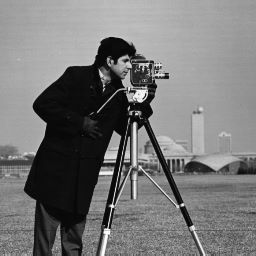
\includegraphics{images/cameraman.jpg}
\caption{camera man image}
\end{figure}

    \hypertarget{a-implementation-of-canny-edge-detector-algorithm}{%
\subsubsection{1.A Implementation of Canny Edge Detector
Algorithm}\label{a-implementation-of-canny-edge-detector-algorithm}}

\begin{enumerate}
\def\labelenumi{\arabic{enumi}.}
\tightlist
\item
  Gaussian Noise
\item
  Gradient Intensification
\item
  Non-Max Suppression
\item
  Thresholding
\end{enumerate}

    \begin{Verbatim}[commandchars=\\\{\}]
{\color{incolor}In [{\color{incolor}1}]:} \PY{k+kn}{import} \PY{n+nn}{cv2}
        \PY{k+kn}{import} \PY{n+nn}{numpy} \PY{k}{as} \PY{n+nn}{np}
        \PY{k+kn}{from} \PY{n+nn}{scipy} \PY{k}{import} \PY{n}{ndimage}
        \PY{k+kn}{from} \PY{n+nn}{PIL} \PY{k}{import} \PY{n}{Image}
        
        \PY{k+kn}{import} \PY{n+nn}{matplotlib}\PY{n+nn}{.}\PY{n+nn}{pyplot} \PY{k}{as} \PY{n+nn}{plt}
        
        \PY{k+kn}{import} \PY{n+nn}{time}
        \PY{o}{\PYZpc{}}\PY{k}{matplotlib} inline
\end{Verbatim}


    \begin{Verbatim}[commandchars=\\\{\}]
{\color{incolor}In [{\color{incolor}87}]:} \PY{k}{def} \PY{n+nf}{open\PYZus{}image}\PY{p}{(}\PY{n}{path}\PY{p}{)}\PY{p}{:}
             \PY{l+s+sd}{\PYZdq{}\PYZdq{}\PYZdq{}}
         \PY{l+s+sd}{    Open an image using PIL library}
         
         \PY{l+s+sd}{    :param path: path to image file\PYZhy{}like}
         \PY{l+s+sd}{    :return: PIL image object}
         \PY{l+s+sd}{    \PYZdq{}\PYZdq{}\PYZdq{}}
             \PY{n}{image} \PY{o}{=} \PY{n}{Image}\PY{o}{.}\PY{n}{open}\PY{p}{(}\PY{n}{path}\PY{p}{)}
             \PY{k}{return} \PY{n}{image}
\end{Verbatim}


    \begin{Verbatim}[commandchars=\\\{\}]
{\color{incolor}In [{\color{incolor}88}]:} \PY{k}{def} \PY{n+nf}{show\PYZus{}image}\PY{p}{(}\PY{n}{image}\PY{p}{,} \PY{n}{cmap}\PY{o}{=}\PY{l+s+s1}{\PYZsq{}}\PY{l+s+s1}{gray}\PY{l+s+s1}{\PYZsq{}}\PY{p}{)}\PY{p}{:}
             \PY{l+s+sd}{\PYZdq{}\PYZdq{}\PYZdq{}}
         \PY{l+s+sd}{    Show PIL image or numpy image in default viewer of OS}
         
         \PY{l+s+sd}{    :param image: image data}
         \PY{l+s+sd}{    :param cmap: color map of input numpy array}
         \PY{l+s+sd}{    :return: None}
         \PY{l+s+sd}{    \PYZdq{}\PYZdq{}\PYZdq{}}
             \PY{k}{if} \PY{n+nb}{str}\PY{p}{(}\PY{n+nb}{type}\PY{p}{(}\PY{n}{image}\PY{p}{)}\PY{p}{)}\PY{o}{.}\PY{n+nf+fm}{\PYZus{}\PYZus{}contains\PYZus{}\PYZus{}}\PY{p}{(}\PY{l+s+s1}{\PYZsq{}}\PY{l+s+s1}{PIL}\PY{l+s+s1}{\PYZsq{}}\PY{p}{)}\PY{p}{:}
                 \PY{n}{image}\PY{o}{.}\PY{n}{show}\PY{p}{(}\PY{p}{)}
             \PY{k}{elif} \PY{n+nb}{str}\PY{p}{(}\PY{n+nb}{type}\PY{p}{(}\PY{n}{image}\PY{p}{)}\PY{p}{)}\PY{o}{.}\PY{n+nf+fm}{\PYZus{}\PYZus{}contains\PYZus{}\PYZus{}}\PY{p}{(}\PY{l+s+s1}{\PYZsq{}}\PY{l+s+s1}{numpy}\PY{l+s+s1}{\PYZsq{}}\PY{p}{)}\PY{p}{:}
                 \PY{k}{if} \PY{n}{cmap}\PY{o}{==}\PY{l+s+s1}{\PYZsq{}}\PY{l+s+s1}{gray}\PY{l+s+s1}{\PYZsq{}}\PY{p}{:}
                     \PY{n}{Image}\PY{o}{.}\PY{n}{fromarray}\PY{p}{(}\PY{n}{np}\PY{o}{.}\PY{n}{uint8}\PY{p}{(}\PY{n}{image}\PY{p}{)}\PY{p}{,} \PY{n}{mode}\PY{o}{=}\PY{l+s+s1}{\PYZsq{}}\PY{l+s+s1}{L}\PY{l+s+s1}{\PYZsq{}}\PY{p}{)}\PY{o}{.}\PY{n}{show}\PY{p}{(}\PY{p}{)}
                 \PY{k}{elif} \PY{n}{cmap} \PY{o}{==} \PY{l+s+s1}{\PYZsq{}}\PY{l+s+s1}{bw}\PY{l+s+s1}{\PYZsq{}}\PY{p}{:}
                     \PY{n}{size} \PY{o}{=} \PY{n}{image}\PY{o}{.}\PY{n}{shape}\PY{p}{[}\PY{p}{:}\PY{p}{:}\PY{o}{\PYZhy{}}\PY{l+m+mi}{1}\PY{p}{]}
                     \PY{n}{data\PYZus{}bytes} \PY{o}{=} \PY{n}{np}\PY{o}{.}\PY{n}{packbits}\PY{p}{(}\PY{n}{image}\PY{p}{,} \PY{n}{axis}\PY{o}{=}\PY{l+m+mi}{1}\PY{p}{)}
                     \PY{n}{Image}\PY{o}{.}\PY{n}{frombytes}\PY{p}{(}\PY{n}{mode}\PY{o}{=}\PY{l+s+s1}{\PYZsq{}}\PY{l+s+s1}{1}\PY{l+s+s1}{\PYZsq{}}\PY{p}{,} \PY{n}{size}\PY{o}{=}\PY{n}{size}\PY{p}{,} \PY{n}{data}\PY{o}{=}\PY{n}{data\PYZus{}bytes}\PY{p}{)}\PY{o}{.}\PY{n}{show}\PY{p}{(}\PY{p}{)}
                 \PY{k}{else}\PY{p}{:}
                     \PY{k}{raise} \PY{n+ne}{ValueError}\PY{p}{(}\PY{l+s+s1}{\PYZsq{}}\PY{l+s+s1}{color map is invalid.}\PY{l+s+s1}{\PYZsq{}}\PY{p}{)}
             \PY{k}{else}\PY{p}{:}
                 \PY{k}{raise} \PY{n+ne}{ValueError}\PY{p}{(}\PY{l+s+s1}{\PYZsq{}}\PY{l+s+s1}{Input t is not valid.}\PY{l+s+s1}{\PYZsq{}}\PY{p}{)}
\end{Verbatim}


    \begin{Verbatim}[commandchars=\\\{\}]
{\color{incolor}In [{\color{incolor}89}]:} \PY{k}{class} \PY{n+nc}{ToGrayscale}\PY{p}{:}
             \PY{l+s+sd}{\PYZdq{}\PYZdq{}\PYZdq{}}
         \PY{l+s+sd}{    Get and PIL image or numpy n\PYZhy{}dim array as image and convert it to grayscale image}
         \PY{l+s+sd}{    \PYZdq{}\PYZdq{}\PYZdq{}}
         
             \PY{k}{def} \PY{n+nf}{\PYZus{}\PYZus{}init\PYZus{}\PYZus{}}\PY{p}{(}\PY{n+nb+bp}{self}\PY{p}{)}\PY{p}{:}
                 \PY{k}{pass}
         
             \PY{k}{def} \PY{n+nf}{\PYZus{}\PYZus{}call\PYZus{}\PYZus{}}\PY{p}{(}\PY{n+nb+bp}{self}\PY{p}{,} \PY{n}{image}\PY{p}{)}\PY{p}{:}
                 \PY{l+s+sd}{\PYZdq{}\PYZdq{}\PYZdq{}}
         \PY{l+s+sd}{        Get and PIL image or numpy n\PYZhy{}dim array as image and convert it to grayscale image}
         
         \PY{l+s+sd}{        :param image: input image data}
         \PY{l+s+sd}{        :return: Grayscale image of input type}
         \PY{l+s+sd}{        \PYZdq{}\PYZdq{}\PYZdq{}}
                 \PY{k}{if} \PY{n+nb}{str}\PY{p}{(}\PY{n+nb}{type}\PY{p}{(}\PY{n}{image}\PY{p}{)}\PY{p}{)}\PY{o}{.}\PY{n+nf+fm}{\PYZus{}\PYZus{}contains\PYZus{}\PYZus{}}\PY{p}{(}\PY{l+s+s1}{\PYZsq{}}\PY{l+s+s1}{PIL}\PY{l+s+s1}{\PYZsq{}}\PY{p}{)}\PY{p}{:}
                     \PY{n}{image} \PY{o}{=} \PY{n}{image}\PY{o}{.}\PY{n}{convert}\PY{p}{(}\PY{l+s+s1}{\PYZsq{}}\PY{l+s+s1}{L}\PY{l+s+s1}{\PYZsq{}}\PY{p}{)}
                 \PY{k}{elif} \PY{n+nb}{str}\PY{p}{(}\PY{n+nb}{type}\PY{p}{(}\PY{n}{image}\PY{p}{)}\PY{p}{)}\PY{o}{.}\PY{n+nf+fm}{\PYZus{}\PYZus{}contains\PYZus{}\PYZus{}}\PY{p}{(}\PY{l+s+s1}{\PYZsq{}}\PY{l+s+s1}{numpy}\PY{l+s+s1}{\PYZsq{}}\PY{p}{)}\PY{p}{:}
                     \PY{n}{image} \PY{o}{=} \PY{n}{np}\PY{o}{.}\PY{n}{dot}\PY{p}{(}\PY{n}{image}\PY{p}{[}\PY{o}{.}\PY{o}{.}\PY{o}{.}\PY{p}{,} \PY{p}{:}\PY{l+m+mi}{3}\PY{p}{]}\PY{p}{,} \PY{p}{[}\PY{l+m+mf}{0.2989}\PY{p}{,} \PY{l+m+mf}{0.5870}\PY{p}{,} \PY{l+m+mf}{0.1140}\PY{p}{]}\PY{p}{)}
                 \PY{k}{else}\PY{p}{:}
                     \PY{k}{raise} \PY{n+ne}{ValueError}\PY{p}{(}\PY{l+s+s1}{\PYZsq{}}\PY{l+s+s1}{Input type is not valid.}\PY{l+s+s1}{\PYZsq{}}\PY{p}{)}
                 \PY{k}{return} \PY{n}{image}
\end{Verbatim}


    \hypertarget{a.a-gaussian-noise}{%
\paragraph{1.A.a Gaussian Noise}\label{a.a-gaussian-noise}}

    \begin{Verbatim}[commandchars=\\\{\}]
{\color{incolor}In [{\color{incolor}90}]:} \PY{k}{class} \PY{n+nc}{GaussianNoise}\PY{p}{:}
             \PY{k}{def} \PY{n+nf}{\PYZus{}\PYZus{}init\PYZus{}\PYZus{}}\PY{p}{(}\PY{n+nb+bp}{self}\PY{p}{,} \PY{n}{size}\PY{o}{=}\PY{l+m+mi}{5}\PY{p}{,} \PY{n}{std}\PY{o}{=}\PY{l+m+mi}{1}\PY{p}{)}\PY{p}{:}
                 \PY{n+nb+bp}{self}\PY{o}{.}\PY{n}{size} \PY{o}{=} \PY{n}{size}
                 \PY{n+nb+bp}{self}\PY{o}{.}\PY{n}{std} \PY{o}{=} \PY{n}{std}
         
             \PY{k}{def} \PY{n+nf}{\PYZus{}gaussian}\PY{p}{(}\PY{n+nb+bp}{self}\PY{p}{,} \PY{n}{r2}\PY{p}{)}\PY{p}{:}
                 \PY{l+s+sd}{\PYZdq{}\PYZdq{}\PYZdq{}}
         \PY{l+s+sd}{        Sample one instance from gaussian distribution regarding}
         \PY{l+s+sd}{        given squared\PYZhy{}distance:r2, standard\PYZhy{}deviation:std and general\PYZhy{}constant:k}
         
         \PY{l+s+sd}{        :param r: squared distance from center of gaussian distribution}
         \PY{l+s+sd}{        :param std: standard deviation}
         
         \PY{l+s+sd}{        :return: A sampled number obtained from gaussian}
         \PY{l+s+sd}{        \PYZdq{}\PYZdq{}\PYZdq{}}
                 \PY{k}{return} \PY{n}{np}\PY{o}{.}\PY{n}{exp}\PY{p}{(}\PY{o}{\PYZhy{}}\PY{n}{r2}\PY{o}{/}\PY{p}{(}\PY{l+m+mf}{2.}\PY{o}{*}\PY{n+nb+bp}{self}\PY{o}{.}\PY{n}{std}\PY{o}{*}\PY{o}{*}\PY{l+m+mi}{2}\PY{p}{)}\PY{p}{)} \PY{o}{/} \PY{p}{(}\PY{l+m+mf}{2.}\PY{o}{*}\PY{n}{np}\PY{o}{.}\PY{n}{pi}\PY{o}{*}\PY{n+nb+bp}{self}\PY{o}{.}\PY{n}{std}\PY{o}{*}\PY{o}{*}\PY{l+m+mi}{2}\PY{p}{)}
             
             \PY{k}{def} \PY{n+nf}{\PYZus{}gaussian\PYZus{}kernel}\PY{p}{(}\PY{n+nb+bp}{self}\PY{p}{)}\PY{p}{:}
                 \PY{l+s+sd}{\PYZdq{}\PYZdq{}\PYZdq{}}
         \PY{l+s+sd}{        Creates a gaussian kernel regarding given size and std.}
         \PY{l+s+sd}{        Note that to define interval with respect to the size, }
         \PY{l+s+sd}{        I used linear space sampling which may has}
         \PY{l+s+sd}{        lower accuracy from renowned libraries.}
         
         \PY{l+s+sd}{        :param std: standard deviation value}
         \PY{l+s+sd}{        :param size: size of the output kernel}
         \PY{l+s+sd}{        :return: A gaussian kernel with size of (size*size)}
         \PY{l+s+sd}{        \PYZdq{}\PYZdq{}\PYZdq{}}
                 \PY{n+nb+bp}{self}\PY{o}{.}\PY{n}{size} \PY{o}{=} \PY{n+nb}{int}\PY{p}{(}\PY{n+nb+bp}{self}\PY{o}{.}\PY{n}{size}\PY{p}{)} \PY{o}{/}\PY{o}{/} \PY{l+m+mi}{2}
                 \PY{n}{x}\PY{p}{,} \PY{n}{y} \PY{o}{=} \PY{n}{np}\PY{o}{.}\PY{n}{mgrid}\PY{p}{[}\PY{o}{\PYZhy{}}\PY{n+nb+bp}{self}\PY{o}{.}\PY{n}{size}\PY{p}{:}\PY{n+nb+bp}{self}\PY{o}{.}\PY{n}{size}\PY{o}{+}\PY{l+m+mi}{1}\PY{p}{,} \PY{o}{\PYZhy{}}\PY{n+nb+bp}{self}\PY{o}{.}\PY{n}{size}\PY{p}{:}\PY{n+nb+bp}{self}\PY{o}{.}\PY{n}{size}\PY{o}{+}\PY{l+m+mi}{1}\PY{p}{]}
                 \PY{n}{distance} \PY{o}{=} \PY{n}{x}\PY{o}{*}\PY{o}{*}\PY{l+m+mi}{2}\PY{o}{+} \PY{n}{y}\PY{o}{*}\PY{o}{*}\PY{l+m+mi}{2}
                 \PY{n}{kernel} \PY{o}{=} \PY{n+nb+bp}{self}\PY{o}{.}\PY{n}{\PYZus{}gaussian}\PY{p}{(}\PY{n}{r2}\PY{o}{=}\PY{n}{distance}\PY{p}{)}
                 \PY{k}{return} \PY{n}{kernel}
             
             \PY{k}{def} \PY{n+nf}{\PYZus{}\PYZus{}call\PYZus{}\PYZus{}}\PY{p}{(}\PY{n+nb+bp}{self}\PY{p}{,} \PY{n}{image}\PY{p}{)}\PY{p}{:}
                 \PY{l+s+sd}{\PYZdq{}\PYZdq{}\PYZdq{}}
         \PY{l+s+sd}{        Applies gaussian noise on the given image}
         
         \PY{l+s+sd}{        :param image: Input image in grayscale mode numpy ndarray or cv2 image}
         \PY{l+s+sd}{        :param size: Size of the gaussian kernel}
         \PY{l+s+sd}{        :param std: Standard deviation value for gaussian kernel}
         \PY{l+s+sd}{        \PYZdq{}\PYZdq{}\PYZdq{}}
         
                 \PY{k}{return} \PY{n}{ndimage}\PY{o}{.}\PY{n}{convolve}\PY{p}{(}\PY{n}{image}\PY{p}{,} \PY{n+nb+bp}{self}\PY{o}{.}\PY{n}{\PYZus{}gaussian\PYZus{}kernel}\PY{p}{(}\PY{p}{)}\PY{p}{)}
\end{Verbatim}


    \begin{Verbatim}[commandchars=\\\{\}]
{\color{incolor}In [{\color{incolor}91}]:} \PY{n}{image} \PY{o}{=} \PY{n}{cv2}\PY{o}{.}\PY{n}{imread}\PY{p}{(}\PY{l+s+s1}{\PYZsq{}}\PY{l+s+s1}{images/cameraman.jpg}\PY{l+s+s1}{\PYZsq{}}\PY{p}{,} \PY{n}{cv2}\PY{o}{.}\PY{n}{IMREAD\PYZus{}GRAYSCALE}\PY{p}{)}
         \PY{n}{gaussian\PYZus{}noise} \PY{o}{=} \PY{n}{GaussianNoise}\PY{p}{(}\PY{p}{)}
         \PY{n}{image\PYZus{}blurred} \PY{o}{=} \PY{n}{gaussian\PYZus{}noise}\PY{p}{(}\PY{n}{image}\PY{p}{)}
         
         \PY{c+c1}{\PYZsh{} plotting}
         \PY{n}{fig}\PY{p}{,} \PY{n}{ax} \PY{o}{=} \PY{n}{plt}\PY{o}{.}\PY{n}{subplots}\PY{p}{(}\PY{n}{nrows}\PY{o}{=}\PY{l+m+mi}{1}\PY{p}{,} \PY{n}{ncols}\PY{o}{=}\PY{l+m+mi}{2}\PY{p}{,} \PY{n}{figsize}\PY{o}{=}\PY{p}{(}\PY{l+m+mi}{20}\PY{p}{,} \PY{l+m+mi}{15}\PY{p}{)}\PY{p}{)}
         \PY{n}{ax}\PY{p}{[}\PY{l+m+mi}{0}\PY{p}{]}\PY{o}{.}\PY{n}{set\PYZus{}title}\PY{p}{(}\PY{l+s+s1}{\PYZsq{}}\PY{l+s+s1}{original}\PY{l+s+s1}{\PYZsq{}}\PY{p}{)}
         \PY{n}{ax}\PY{p}{[}\PY{l+m+mi}{1}\PY{p}{]}\PY{o}{.}\PY{n}{set\PYZus{}title}\PY{p}{(}\PY{l+s+s1}{\PYZsq{}}\PY{l+s+s1}{blurred}\PY{l+s+s1}{\PYZsq{}}\PY{p}{)}
         \PY{n}{ax}\PY{p}{[}\PY{l+m+mi}{0}\PY{p}{]}\PY{o}{.}\PY{n}{imshow}\PY{p}{(}\PY{n}{image}\PY{p}{,} \PY{n}{cmap}\PY{o}{=}\PY{l+s+s1}{\PYZsq{}}\PY{l+s+s1}{gray}\PY{l+s+s1}{\PYZsq{}}\PY{p}{)}
         \PY{n}{ax}\PY{p}{[}\PY{l+m+mi}{1}\PY{p}{]}\PY{o}{.}\PY{n}{imshow}\PY{p}{(}\PY{n}{image\PYZus{}blurred}\PY{p}{,} \PY{n}{cmap}\PY{o}{=}\PY{l+s+s1}{\PYZsq{}}\PY{l+s+s1}{gray}\PY{l+s+s1}{\PYZsq{}}\PY{p}{)}
\end{Verbatim}


\begin{Verbatim}[commandchars=\\\{\}]
{\color{outcolor}Out[{\color{outcolor}91}]:} <matplotlib.image.AxesImage at 0x2505b44d5f8>
\end{Verbatim}
            
    \begin{center}
    \adjustimage{max size={0.9\linewidth}{0.9\paperheight}}{output_9_1.png}
    \end{center}
    { \hspace*{\fill} \\}
    
    \hypertarget{a.b-gradient-intensity}{%
\paragraph{1.A.b Gradient Intensity}\label{a.b-gradient-intensity}}

    \begin{Verbatim}[commandchars=\\\{\}]
{\color{incolor}In [{\color{incolor}92}]:} \PY{k}{class} \PY{n+nc}{GradientIntensity}\PY{p}{:}
             \PY{l+s+sd}{\PYZdq{}\PYZdq{}\PYZdq{}}
         \PY{l+s+sd}{    We use Sobel filters to convolve over image (numpy ndarray) to calculate gradient intensity on both}
         \PY{l+s+sd}{    horizontal and vertical directions. Finally returns magnitude G and slope theta as follows:}
         
         \PY{l+s+sd}{    G = sqrt(Ix\PYZca{}2 + Iy\PYZca{}2)}
         
         \PY{l+s+sd}{    theta = arctan(Ix/Iy)}
         
         \PY{l+s+sd}{    We use these Sobel filters as default:}
         
         \PY{l+s+sd}{    Kx =}
         \PY{l+s+sd}{    [[\PYZhy{}1 0 1],}
         \PY{l+s+sd}{    [\PYZhy{}2 0 2],}
         \PY{l+s+sd}{    [\PYZhy{}1 0 1]]}
         
         \PY{l+s+sd}{    Ky =}
         \PY{l+s+sd}{    [[1 2 1],}
         \PY{l+s+sd}{    [0 0 0],}
         \PY{l+s+sd}{    [\PYZhy{}1 \PYZhy{}2 \PYZhy{}1]]}
         
         \PY{l+s+sd}{    \PYZdq{}\PYZdq{}\PYZdq{}}
         
             \PY{k}{def} \PY{n+nf}{\PYZus{}\PYZus{}init\PYZus{}\PYZus{}}\PY{p}{(}\PY{n+nb+bp}{self}\PY{p}{,} \PY{n}{hf}\PY{o}{=}\PY{k+kc}{None}\PY{p}{,} \PY{n}{vf}\PY{o}{=}\PY{k+kc}{None}\PY{p}{,} \PY{n}{init}\PY{o}{=}\PY{k+kc}{True}\PY{p}{)}\PY{p}{:}
                 \PY{l+s+sd}{\PYZdq{}\PYZdq{}\PYZdq{}}
         \PY{l+s+sd}{        Initialize filters}
         
         \PY{l+s+sd}{        :param hf: Horizontal filter matrix \PYZhy{}\PYZgt{} numpy ndarray}
         \PY{l+s+sd}{        :param vf: Vertical filter matrix \PYZhy{}\PYZgt{} numpy ndarray}
         \PY{l+s+sd}{        :param init: whether initialize Sobel filters or initialize using user provided input \PYZhy{}\PYZgt{} default Sobel}
         \PY{l+s+sd}{        \PYZdq{}\PYZdq{}\PYZdq{}}
         
                 \PY{k}{if} \PY{o+ow}{not} \PY{n}{init}\PY{p}{:}
                     \PY{n+nb+bp}{self}\PY{o}{.}\PY{n}{hf} \PY{o}{=} \PY{n}{hf}
                     \PY{n+nb+bp}{self}\PY{o}{.}\PY{n}{vf} \PY{o}{=} \PY{n}{vf}
                 \PY{k}{else}\PY{p}{:}
                     \PY{n+nb+bp}{self}\PY{o}{.}\PY{n}{hf} \PY{o}{=} \PY{n}{np}\PY{o}{.}\PY{n}{array}\PY{p}{(}
                         \PY{p}{[}\PY{p}{[}\PY{o}{\PYZhy{}}\PY{l+m+mi}{1}\PY{p}{,} \PY{l+m+mi}{0}\PY{p}{,} \PY{l+m+mi}{1}\PY{p}{]}\PY{p}{,}
                          \PY{p}{[}\PY{o}{\PYZhy{}}\PY{l+m+mi}{2}\PY{p}{,} \PY{l+m+mi}{0}\PY{p}{,} \PY{l+m+mi}{2}\PY{p}{]}\PY{p}{,}
                          \PY{p}{[}\PY{o}{\PYZhy{}}\PY{l+m+mi}{1}\PY{p}{,} \PY{l+m+mi}{0}\PY{p}{,} \PY{l+m+mi}{1}\PY{p}{]}\PY{p}{]}\PY{p}{)}
         
                     \PY{n+nb+bp}{self}\PY{o}{.}\PY{n}{vf} \PY{o}{=} \PY{n}{np}\PY{o}{.}\PY{n}{array}\PY{p}{(}
                         \PY{p}{[}\PY{p}{[}\PY{l+m+mi}{1}\PY{p}{,} \PY{l+m+mi}{2}\PY{p}{,} \PY{l+m+mi}{1}\PY{p}{]}\PY{p}{,}
                          \PY{p}{[}\PY{l+m+mi}{0}\PY{p}{,} \PY{l+m+mi}{0}\PY{p}{,} \PY{l+m+mi}{0}\PY{p}{]}\PY{p}{,}
                          \PY{p}{[}\PY{o}{\PYZhy{}}\PY{l+m+mi}{1}\PY{p}{,} \PY{o}{\PYZhy{}}\PY{l+m+mi}{2}\PY{p}{,} \PY{o}{\PYZhy{}}\PY{l+m+mi}{1}\PY{p}{]}\PY{p}{]}\PY{p}{)}
         
             \PY{k}{def} \PY{n+nf}{\PYZus{}\PYZus{}call\PYZus{}\PYZus{}}\PY{p}{(}\PY{n+nb+bp}{self}\PY{p}{,} \PY{n}{x}\PY{p}{)}\PY{p}{:}
                 \PY{k}{if} \PY{o+ow}{not} \PY{n+nb}{str}\PY{p}{(}\PY{n+nb}{type}\PY{p}{(}\PY{n}{x}\PY{p}{)}\PY{p}{)}\PY{o}{.}\PY{n+nf+fm}{\PYZus{}\PYZus{}contains\PYZus{}\PYZus{}}\PY{p}{(}\PY{l+s+s1}{\PYZsq{}}\PY{l+s+s1}{numpy}\PY{l+s+s1}{\PYZsq{}}\PY{p}{)}\PY{p}{:}
                     \PY{k}{raise} \PY{n+ne}{ValueError}\PY{p}{(}\PY{l+s+s1}{\PYZsq{}}\PY{l+s+s1}{Invalid input. Please provide numpy ndarray image.}\PY{l+s+s1}{\PYZsq{}}\PY{p}{)}
                 \PY{n}{Ix} \PY{o}{=} \PY{n}{ndimage}\PY{o}{.}\PY{n}{filters}\PY{o}{.}\PY{n}{convolve}\PY{p}{(}\PY{n}{x}\PY{p}{,} \PY{n+nb+bp}{self}\PY{o}{.}\PY{n}{hf}\PY{p}{)}
                 \PY{n}{Iy} \PY{o}{=} \PY{n}{ndimage}\PY{o}{.}\PY{n}{filters}\PY{o}{.}\PY{n}{convolve}\PY{p}{(}\PY{n}{x}\PY{p}{,} \PY{n+nb+bp}{self}\PY{o}{.}\PY{n}{vf}\PY{p}{)}
         
                 \PY{n}{G} \PY{o}{=} \PY{n}{np}\PY{o}{.}\PY{n}{sqrt}\PY{p}{(}\PY{n}{np}\PY{o}{.}\PY{n}{power}\PY{p}{(}\PY{n}{Ix}\PY{p}{,} \PY{l+m+mi}{2}\PY{p}{)}  \PY{o}{+} \PY{n}{np}\PY{o}{.}\PY{n}{power}\PY{p}{(}\PY{n}{Iy}\PY{p}{,} \PY{l+m+mi}{2}\PY{p}{)}\PY{p}{)}
                 \PY{n}{G} \PY{o}{=} \PY{n}{G} \PY{o}{/} \PY{n}{G}\PY{o}{.}\PY{n}{max}\PY{p}{(}\PY{p}{)} \PY{o}{*} \PY{l+m+mi}{255}
                 \PY{n}{theta} \PY{o}{=} \PY{n}{np}\PY{o}{.}\PY{n}{arctan2}\PY{p}{(}\PY{n}{Iy}\PY{p}{,} \PY{n}{Ix}\PY{p}{)}
         
                 \PY{k}{return} \PY{n}{G}\PY{p}{,} \PY{n}{theta}
\end{Verbatim}


    \begin{Verbatim}[commandchars=\\\{\}]
{\color{incolor}In [{\color{incolor}93}]:} \PY{c+c1}{\PYZsh{} image = cv2.imread(\PYZsq{}images/cameraman.jpg\PYZsq{}, cv2.IMREAD\PYZus{}GRAYSCALE)}
         \PY{n}{to\PYZus{}grayscale} \PY{o}{=} \PY{n}{ToGrayscale}\PY{p}{(}\PY{p}{)}
         \PY{n}{image} \PY{o}{=} \PY{n}{np}\PY{o}{.}\PY{n}{array}\PY{p}{(}\PY{n}{to\PYZus{}grayscale}\PY{p}{(}\PY{n}{open\PYZus{}image}\PY{p}{(}\PY{l+s+s1}{\PYZsq{}}\PY{l+s+s1}{images/cameraman.jpg}\PY{l+s+s1}{\PYZsq{}}\PY{p}{)}\PY{p}{)}\PY{p}{,} \PY{n}{dtype}\PY{o}{=}\PY{n+nb}{float}\PY{p}{)}  \PY{c+c1}{\PYZsh{} this \PYZsq{}float\PYZsq{} took me 7 hours!}
         \PY{n}{gaussian\PYZus{}noise} \PY{o}{=} \PY{n}{GaussianNoise}\PY{p}{(}\PY{p}{)}
         \PY{n}{image\PYZus{}blurred} \PY{o}{=} \PY{n}{gaussian\PYZus{}noise}\PY{p}{(}\PY{n}{image}\PY{p}{)}
         \PY{n}{gradient\PYZus{}intensity} \PY{o}{=} \PY{n}{GradientIntensity}\PY{p}{(}\PY{p}{)}
         \PY{n}{image\PYZus{}grad}\PY{p}{,} \PY{n}{image\PYZus{}theta} \PY{o}{=} \PY{n}{gradient\PYZus{}intensity}\PY{p}{(}\PY{n}{image\PYZus{}blurred}\PY{p}{)}
         
         \PY{c+c1}{\PYZsh{} plotting}
         \PY{n}{fig}\PY{p}{,} \PY{n}{ax} \PY{o}{=} \PY{n}{plt}\PY{o}{.}\PY{n}{subplots}\PY{p}{(}\PY{n}{nrows}\PY{o}{=}\PY{l+m+mi}{1}\PY{p}{,} \PY{n}{ncols}\PY{o}{=}\PY{l+m+mi}{3}\PY{p}{,} \PY{n}{figsize}\PY{o}{=}\PY{p}{(}\PY{l+m+mi}{20}\PY{p}{,} \PY{l+m+mi}{15}\PY{p}{)}\PY{p}{)}
         \PY{n}{ax}\PY{p}{[}\PY{l+m+mi}{0}\PY{p}{]}\PY{o}{.}\PY{n}{set\PYZus{}title}\PY{p}{(}\PY{l+s+s1}{\PYZsq{}}\PY{l+s+s1}{blurred}\PY{l+s+s1}{\PYZsq{}}\PY{p}{)}
         \PY{n}{ax}\PY{p}{[}\PY{l+m+mi}{1}\PY{p}{]}\PY{o}{.}\PY{n}{set\PYZus{}title}\PY{p}{(}\PY{l+s+s1}{\PYZsq{}}\PY{l+s+s1}{grad}\PY{l+s+s1}{\PYZsq{}}\PY{p}{)}
         \PY{n}{ax}\PY{p}{[}\PY{l+m+mi}{2}\PY{p}{]}\PY{o}{.}\PY{n}{set\PYZus{}title}\PY{p}{(}\PY{l+s+s1}{\PYZsq{}}\PY{l+s+s1}{theta}\PY{l+s+s1}{\PYZsq{}}\PY{p}{)}
         \PY{n}{ax}\PY{p}{[}\PY{l+m+mi}{0}\PY{p}{]}\PY{o}{.}\PY{n}{imshow}\PY{p}{(}\PY{n}{image\PYZus{}blurred}\PY{p}{,} \PY{n}{cmap}\PY{o}{=}\PY{l+s+s1}{\PYZsq{}}\PY{l+s+s1}{gray}\PY{l+s+s1}{\PYZsq{}}\PY{p}{)}
         \PY{n}{ax}\PY{p}{[}\PY{l+m+mi}{1}\PY{p}{]}\PY{o}{.}\PY{n}{imshow}\PY{p}{(}\PY{n}{image\PYZus{}grad}\PY{p}{,} \PY{n}{cmap}\PY{o}{=}\PY{l+s+s1}{\PYZsq{}}\PY{l+s+s1}{gray}\PY{l+s+s1}{\PYZsq{}}\PY{p}{)}
         \PY{n}{ax}\PY{p}{[}\PY{l+m+mi}{2}\PY{p}{]}\PY{o}{.}\PY{n}{imshow}\PY{p}{(}\PY{n}{image\PYZus{}theta}\PY{p}{,} \PY{n}{cmap}\PY{o}{=}\PY{l+s+s1}{\PYZsq{}}\PY{l+s+s1}{gray}\PY{l+s+s1}{\PYZsq{}}\PY{p}{)}
\end{Verbatim}


\begin{Verbatim}[commandchars=\\\{\}]
{\color{outcolor}Out[{\color{outcolor}93}]:} <matplotlib.image.AxesImage at 0x2505b4f1048>
\end{Verbatim}
            
    \begin{center}
    \adjustimage{max size={0.9\linewidth}{0.9\paperheight}}{output_12_1.png}
    \end{center}
    { \hspace*{\fill} \\}
    
    \hypertarget{a.c-non-max-suppression}{%
\paragraph{1.A.c Non-Max Suppression}\label{a.c-non-max-suppression}}

    \begin{Verbatim}[commandchars=\\\{\}]
{\color{incolor}In [{\color{incolor}94}]:} \PY{k}{class} \PY{n+nc}{NonMaxSuppression}\PY{p}{:}
             \PY{l+s+sd}{\PYZdq{}\PYZdq{}\PYZdq{}}
         \PY{l+s+sd}{    Get gradient of image w.r.t the filters and degree of gradients (theta) and keep}
         \PY{l+s+sd}{    most intensified pixel in each direction.}
         \PY{l+s+sd}{    Note: d\PYZus{}prime = d\PYZhy{}180}
         \PY{l+s+sd}{    \PYZdq{}\PYZdq{}\PYZdq{}}
         
             \PY{k}{def} \PY{n+nf}{\PYZus{}\PYZus{}init\PYZus{}\PYZus{}}\PY{p}{(}\PY{n+nb+bp}{self}\PY{p}{)}\PY{p}{:}
                 \PY{k}{pass}
         
             \PY{k}{def} \PY{n+nf}{\PYZus{}\PYZus{}call\PYZus{}\PYZus{}}\PY{p}{(}\PY{n+nb+bp}{self}\PY{p}{,} \PY{n}{grad\PYZus{}img}\PY{p}{,} \PY{n}{grad\PYZus{}dir}\PY{p}{)}\PY{p}{:}
                 \PY{l+s+sd}{\PYZdq{}\PYZdq{}\PYZdq{}}
         \PY{l+s+sd}{        Get non\PYZhy{}max suppressed image by preserving most intensified pixels}
         
         \PY{l+s+sd}{        :param grad\PYZus{}img: Gradient image gathered by convolving filters on original image \PYZhy{}\PYZgt{} numpy ndarray}
         \PY{l+s+sd}{        :param grad\PYZus{}dir: Gradient directions gathered by convolving filters on original image \PYZhy{}\PYZgt{} numpy ndarray}
         \PY{l+s+sd}{        :return: Soft\PYZhy{}edge numpy ndarray image}
         \PY{l+s+sd}{        \PYZdq{}\PYZdq{}\PYZdq{}}
         
                 \PY{n}{z} \PY{o}{=} \PY{n}{np}\PY{o}{.}\PY{n}{zeros}\PY{p}{(}\PY{n}{shape}\PY{o}{=}\PY{n}{grad\PYZus{}img}\PY{o}{.}\PY{n}{shape}\PY{p}{,} \PY{n}{dtype}\PY{o}{=}\PY{n}{np}\PY{o}{.}\PY{n}{int32}\PY{p}{)}
         
                 \PY{k}{for} \PY{n}{h} \PY{o+ow}{in} \PY{n+nb}{range}\PY{p}{(}\PY{n}{grad\PYZus{}img}\PY{o}{.}\PY{n}{shape}\PY{p}{[}\PY{l+m+mi}{0}\PY{p}{]}\PY{p}{)}\PY{p}{:}
                     \PY{k}{for} \PY{n}{v} \PY{o+ow}{in} \PY{n+nb}{range}\PY{p}{(}\PY{n}{grad\PYZus{}img}\PY{o}{.}\PY{n}{shape}\PY{p}{[}\PY{l+m+mi}{1}\PY{p}{]}\PY{p}{)}\PY{p}{:}
                         \PY{n}{degree} \PY{o}{=} \PY{n+nb+bp}{self}\PY{o}{.}\PY{n}{\PYZus{}\PYZus{}angle\PYZus{}\PYZus{}}\PY{p}{(}\PY{n}{grad\PYZus{}dir}\PY{p}{[}\PY{n}{h}\PY{p}{]}\PY{p}{[}\PY{n}{v}\PY{p}{]}\PY{p}{)}
         
                         \PY{k}{try}\PY{p}{:}
                             \PY{k}{if} \PY{n}{degree} \PY{o}{==} \PY{l+m+mi}{0}\PY{p}{:}
                                 \PY{k}{if} \PY{n}{grad\PYZus{}img}\PY{p}{[}\PY{n}{h}\PY{p}{]}\PY{p}{[}\PY{n}{v}\PY{p}{]} \PY{o}{\PYZgt{}}\PY{o}{=} \PY{n}{grad\PYZus{}img}\PY{p}{[}\PY{n}{h}\PY{p}{]}\PY{p}{[}\PY{n}{v} \PY{o}{\PYZhy{}} \PY{l+m+mi}{1}\PY{p}{]} \PY{o+ow}{and} \PY{n}{grad\PYZus{}img}\PY{p}{[}\PY{n}{h}\PY{p}{]}\PY{p}{[}\PY{n}{v}\PY{p}{]} \PY{o}{\PYZgt{}}\PY{o}{=} \PY{n}{grad\PYZus{}img}\PY{p}{[}\PY{n}{h}\PY{p}{]}\PY{p}{[}\PY{n}{v} \PY{o}{+} \PY{l+m+mi}{1}\PY{p}{]}\PY{p}{:}
                                     \PY{n}{z}\PY{p}{[}\PY{n}{h}\PY{p}{]}\PY{p}{[}\PY{n}{v}\PY{p}{]} \PY{o}{=} \PY{n}{grad\PYZus{}img}\PY{p}{[}\PY{n}{h}\PY{p}{]}\PY{p}{[}\PY{n}{v}\PY{p}{]}
                             \PY{k}{elif} \PY{n}{degree} \PY{o}{==} \PY{l+m+mi}{45}\PY{p}{:}
                                 \PY{k}{if} \PY{n}{grad\PYZus{}img}\PY{p}{[}\PY{n}{h}\PY{p}{]}\PY{p}{[}\PY{n}{v}\PY{p}{]} \PY{o}{\PYZgt{}}\PY{o}{=} \PY{n}{grad\PYZus{}img}\PY{p}{[}\PY{n}{h} \PY{o}{\PYZhy{}} \PY{l+m+mi}{1}\PY{p}{]}\PY{p}{[}\PY{n}{v} \PY{o}{+} \PY{l+m+mi}{1}\PY{p}{]} \PY{o+ow}{and} \PY{n}{grad\PYZus{}img}\PY{p}{[}\PY{n}{h}\PY{p}{]}\PY{p}{[}\PY{n}{v}\PY{p}{]} \PY{o}{\PYZgt{}}\PY{o}{=} \PY{n}{grad\PYZus{}img}\PY{p}{[}\PY{n}{h} \PY{o}{+} \PY{l+m+mi}{1}\PY{p}{]}\PY{p}{[}\PY{n}{v} \PY{o}{\PYZhy{}} \PY{l+m+mi}{1}\PY{p}{]}\PY{p}{:}
                                     \PY{n}{z}\PY{p}{[}\PY{n}{h}\PY{p}{]}\PY{p}{[}\PY{n}{v}\PY{p}{]} \PY{o}{=} \PY{n}{grad\PYZus{}img}\PY{p}{[}\PY{n}{h}\PY{p}{]}\PY{p}{[}\PY{n}{v}\PY{p}{]}
                             \PY{k}{elif} \PY{n}{degree} \PY{o}{==} \PY{l+m+mi}{90}\PY{p}{:}
                                 \PY{k}{if} \PY{n}{grad\PYZus{}img}\PY{p}{[}\PY{n}{h}\PY{p}{]}\PY{p}{[}\PY{n}{v}\PY{p}{]} \PY{o}{\PYZgt{}}\PY{o}{=} \PY{n}{grad\PYZus{}img}\PY{p}{[}\PY{n}{h} \PY{o}{\PYZhy{}} \PY{l+m+mi}{1}\PY{p}{]}\PY{p}{[}\PY{n}{v}\PY{p}{]} \PY{o+ow}{and} \PY{n}{grad\PYZus{}img}\PY{p}{[}\PY{n}{h}\PY{p}{]}\PY{p}{[}\PY{n}{v}\PY{p}{]} \PY{o}{\PYZgt{}}\PY{o}{=} \PY{n}{grad\PYZus{}img}\PY{p}{[}\PY{n}{h} \PY{o}{+} \PY{l+m+mi}{1}\PY{p}{]}\PY{p}{[}\PY{n}{v}\PY{p}{]}\PY{p}{:}
                                     \PY{n}{z}\PY{p}{[}\PY{n}{h}\PY{p}{]}\PY{p}{[}\PY{n}{v}\PY{p}{]} \PY{o}{=} \PY{n}{grad\PYZus{}img}\PY{p}{[}\PY{n}{h}\PY{p}{]}\PY{p}{[}\PY{n}{v}\PY{p}{]}
                             \PY{k}{elif} \PY{n}{degree} \PY{o}{==} \PY{l+m+mi}{135}\PY{p}{:}
                                 \PY{k}{if} \PY{n}{grad\PYZus{}img}\PY{p}{[}\PY{n}{h}\PY{p}{]}\PY{p}{[}\PY{n}{v}\PY{p}{]} \PY{o}{\PYZgt{}}\PY{o}{=} \PY{n}{grad\PYZus{}img}\PY{p}{[}\PY{n}{h} \PY{o}{\PYZhy{}} \PY{l+m+mi}{1}\PY{p}{]}\PY{p}{[}\PY{n}{v} \PY{o}{\PYZhy{}} \PY{l+m+mi}{1}\PY{p}{]} \PY{o+ow}{and} \PY{n}{grad\PYZus{}img}\PY{p}{[}\PY{n}{h}\PY{p}{]}\PY{p}{[}\PY{n}{v}\PY{p}{]} \PY{o}{\PYZgt{}}\PY{o}{=} \PY{n}{grad\PYZus{}img}\PY{p}{[}\PY{n}{h} \PY{o}{+} \PY{l+m+mi}{1}\PY{p}{]}\PY{p}{[}\PY{n}{v} \PY{o}{+} \PY{l+m+mi}{1}\PY{p}{]}\PY{p}{:}
                                     \PY{n}{z}\PY{p}{[}\PY{n}{h}\PY{p}{]}\PY{p}{[}\PY{n}{v}\PY{p}{]} \PY{o}{=} \PY{n}{grad\PYZus{}img}\PY{p}{[}\PY{n}{h}\PY{p}{]}\PY{p}{[}\PY{n}{v}\PY{p}{]}
                         \PY{k}{except} \PY{n+ne}{IndexError} \PY{k}{as} \PY{n}{exc}\PY{p}{:}
                             \PY{c+c1}{\PYZsh{} Handle boundary index errors}
                             \PY{k}{pass}
                 \PY{k}{return} \PY{n}{z}
         
             \PY{n+nd}{@staticmethod}
             \PY{k}{def} \PY{n+nf}{\PYZus{}\PYZus{}angle\PYZus{}\PYZus{}}\PY{p}{(}\PY{n}{a}\PY{p}{)}\PY{p}{:}
                 \PY{l+s+sd}{\PYZdq{}\PYZdq{}\PYZdq{}}
         \PY{l+s+sd}{        Convert gradient directions in radian to 4 possible direction in degree system}
         
         \PY{l+s+sd}{        :param a: Radian value of gradient direction numpy ndarray matrix}
         \PY{l+s+sd}{        :return: A int within \PYZob{}0, 45, 90, 135\PYZcb{}}
         \PY{l+s+sd}{        \PYZdq{}\PYZdq{}\PYZdq{}}
                 \PY{n}{angle} \PY{o}{=} \PY{n}{np}\PY{o}{.}\PY{n}{rad2deg}\PY{p}{(}\PY{n}{a}\PY{p}{)} \PY{o}{\PYZpc{}} \PY{l+m+mi}{180}
                 \PY{k}{if} \PY{p}{(}\PY{l+m+mi}{0} \PY{o}{\PYZlt{}}\PY{o}{=} \PY{n}{angle} \PY{o}{\PYZlt{}} \PY{l+m+mf}{22.5}\PY{p}{)} \PY{o+ow}{or} \PY{p}{(}\PY{l+m+mf}{157.5} \PY{o}{\PYZlt{}}\PY{o}{=} \PY{n}{angle} \PY{o}{\PYZlt{}} \PY{l+m+mi}{180}\PY{p}{)}\PY{p}{:}
                     \PY{n}{angle} \PY{o}{=} \PY{l+m+mi}{0}
                 \PY{k}{elif} \PY{l+m+mf}{22.5} \PY{o}{\PYZlt{}}\PY{o}{=} \PY{n}{angle} \PY{o}{\PYZlt{}} \PY{l+m+mf}{67.5}\PY{p}{:}
                     \PY{n}{angle} \PY{o}{=} \PY{l+m+mi}{45}
                 \PY{k}{elif} \PY{l+m+mf}{67.5} \PY{o}{\PYZlt{}}\PY{o}{=} \PY{n}{angle} \PY{o}{\PYZlt{}} \PY{l+m+mf}{112.5}\PY{p}{:}
                     \PY{n}{angle} \PY{o}{=} \PY{l+m+mi}{90}
                 \PY{k}{elif} \PY{l+m+mf}{112.5} \PY{o}{\PYZlt{}}\PY{o}{=} \PY{n}{angle} \PY{o}{\PYZlt{}} \PY{l+m+mf}{157.5}\PY{p}{:}
                     \PY{n}{angle} \PY{o}{=} \PY{l+m+mi}{135}
                 \PY{k}{return} \PY{n}{angle}
\end{Verbatim}


    \begin{Verbatim}[commandchars=\\\{\}]
{\color{incolor}In [{\color{incolor}98}]:} \PY{n}{non\PYZus{}max\PYZus{}suppression} \PY{o}{=} \PY{n}{NonMaxSuppression}\PY{p}{(}\PY{p}{)}
         \PY{n}{image\PYZus{}non\PYZus{}max} \PY{o}{=} \PY{n}{non\PYZus{}max\PYZus{}suppression}\PY{p}{(}\PY{n}{image\PYZus{}grad}\PY{p}{,} \PY{n}{image\PYZus{}theta}\PY{p}{)}
         
         \PY{c+c1}{\PYZsh{} plotting}
         \PY{n}{fig}\PY{p}{,} \PY{n}{ax} \PY{o}{=} \PY{n}{plt}\PY{o}{.}\PY{n}{subplots}\PY{p}{(}\PY{n}{nrows}\PY{o}{=}\PY{l+m+mi}{1}\PY{p}{,} \PY{n}{ncols}\PY{o}{=}\PY{l+m+mi}{2}\PY{p}{,} \PY{n}{figsize}\PY{o}{=}\PY{p}{(}\PY{l+m+mi}{20}\PY{p}{,} \PY{l+m+mi}{15}\PY{p}{)}\PY{p}{)}
         \PY{n}{ax}\PY{p}{[}\PY{l+m+mi}{0}\PY{p}{]}\PY{o}{.}\PY{n}{imshow}\PY{p}{(}\PY{n}{image\PYZus{}grad}\PY{p}{,} \PY{n}{cmap}\PY{o}{=}\PY{l+s+s1}{\PYZsq{}}\PY{l+s+s1}{gray}\PY{l+s+s1}{\PYZsq{}}\PY{p}{)}
         \PY{n}{ax}\PY{p}{[}\PY{l+m+mi}{1}\PY{p}{]}\PY{o}{.}\PY{n}{imshow}\PY{p}{(}\PY{n}{image\PYZus{}non\PYZus{}max}\PY{p}{,} \PY{n}{cmap}\PY{o}{=}\PY{l+s+s1}{\PYZsq{}}\PY{l+s+s1}{gray}\PY{l+s+s1}{\PYZsq{}}\PY{p}{)}
         \PY{n}{ax}\PY{p}{[}\PY{l+m+mi}{0}\PY{p}{]}\PY{o}{.}\PY{n}{set\PYZus{}title}\PY{p}{(}\PY{l+s+s1}{\PYZsq{}}\PY{l+s+s1}{grad image}\PY{l+s+s1}{\PYZsq{}}\PY{p}{)}
         \PY{n}{ax}\PY{p}{[}\PY{l+m+mi}{1}\PY{p}{]}\PY{o}{.}\PY{n}{set\PYZus{}title}\PY{p}{(}\PY{l+s+s1}{\PYZsq{}}\PY{l+s+s1}{non max suppressed}\PY{l+s+s1}{\PYZsq{}}\PY{p}{)}
         \PY{n}{plt}\PY{o}{.}\PY{n}{show}\PY{p}{(}\PY{p}{)}
\end{Verbatim}


    \begin{center}
    \adjustimage{max size={0.9\linewidth}{0.9\paperheight}}{output_15_0.png}
    \end{center}
    { \hspace*{\fill} \\}
    
    \hypertarget{a.d-thresholding}{%
\paragraph{1.A.d Thresholding}\label{a.d-thresholding}}

    \begin{Verbatim}[commandchars=\\\{\}]
{\color{incolor}In [{\color{incolor}106}]:} \PY{k}{class} \PY{n+nc}{Thresholding}\PY{p}{:}
              \PY{k}{def} \PY{n+nf}{\PYZus{}\PYZus{}init\PYZus{}\PYZus{}}\PY{p}{(}\PY{n+nb+bp}{self}\PY{p}{,} \PY{n}{high\PYZus{}threshold} \PY{o}{=} \PY{l+m+mi}{90}\PY{p}{,} \PY{n}{low\PYZus{}threshold} \PY{o}{=} \PY{l+m+mi}{30}\PY{p}{)}\PY{p}{:}
                  \PY{n+nb+bp}{self}\PY{o}{.}\PY{n}{high\PYZus{}threshold} \PY{o}{=} \PY{n}{high\PYZus{}threshold}
                  \PY{n+nb+bp}{self}\PY{o}{.}\PY{n}{low\PYZus{}threshold} \PY{o}{=} \PY{n}{low\PYZus{}threshold}
                  \PY{n+nb+bp}{self}\PY{o}{.}\PY{n}{weak} \PY{o}{=} \PY{l+m+mi}{29}
                  \PY{n+nb+bp}{self}\PY{o}{.}\PY{n}{strong} \PY{o}{=} \PY{l+m+mi}{255}
                  \PY{n+nb+bp}{self}\PY{o}{.}\PY{n}{flag} \PY{o}{=} \PY{n+nb+bp}{self}\PY{o}{.}\PY{n}{weak}\PY{o}{*}\PY{l+m+mi}{9}
                  
              \PY{k}{def} \PY{n+nf}{\PYZus{}threshold\PYZus{}image}\PY{p}{(}\PY{n+nb+bp}{self}\PY{p}{,} \PY{n}{image}\PY{p}{)}\PY{p}{:}
                  \PY{n}{thresholded} \PY{o}{=} \PY{n}{np}\PY{o}{.}\PY{n}{empty}\PY{p}{(}\PY{n}{image}\PY{o}{.}\PY{n}{shape}\PY{p}{)}
                  \PY{n}{thresholded}\PY{p}{[}\PY{n}{np}\PY{o}{.}\PY{n}{where}\PY{p}{(}\PY{n}{image}\PY{o}{\PYZgt{}}\PY{n+nb+bp}{self}\PY{o}{.}\PY{n}{high\PYZus{}threshold}\PY{p}{)}\PY{p}{]} \PY{o}{=} \PY{n+nb+bp}{self}\PY{o}{.}\PY{n}{strong}
                  \PY{n}{thresholded}\PY{p}{[}\PY{n}{np}\PY{o}{.}\PY{n}{where}\PY{p}{(}\PY{p}{(}\PY{p}{(}\PY{n}{image}\PY{o}{\PYZgt{}}\PY{n+nb+bp}{self}\PY{o}{.}\PY{n}{low\PYZus{}threshold}\PY{p}{)} \PY{o}{\PYZam{}} \PY{p}{(}\PY{n}{image}\PY{o}{\PYZlt{}}\PY{o}{=}\PY{n+nb+bp}{self}\PY{o}{.}\PY{n}{high\PYZus{}threshold}\PY{p}{)}\PY{p}{)}\PY{p}{)}\PY{p}{]} \PY{o}{=} \PY{n+nb+bp}{self}\PY{o}{.}\PY{n}{weak}
                  \PY{k}{return} \PY{n}{thresholded}
              
              \PY{k}{def} \PY{n+nf}{\PYZus{}\PYZus{}call\PYZus{}\PYZus{}}\PY{p}{(}\PY{n+nb+bp}{self}\PY{p}{,} \PY{n}{image}\PY{p}{)}\PY{p}{:}
                  \PY{n}{thresholded} \PY{o}{=} \PY{n+nb+bp}{self}\PY{o}{.}\PY{n}{\PYZus{}threshold\PYZus{}image}\PY{p}{(}\PY{n}{image}\PY{p}{)}
                  \PY{k}{for} \PY{n}{i} \PY{o+ow}{in} \PY{n+nb}{range}\PY{p}{(}\PY{n}{thresholded}\PY{o}{.}\PY{n}{shape}\PY{p}{[}\PY{l+m+mi}{0}\PY{p}{]}\PY{p}{)}\PY{p}{:}
                      \PY{k}{for} \PY{n}{j} \PY{o+ow}{in} \PY{n+nb}{range}\PY{p}{(}\PY{n}{thresholded}\PY{o}{.}\PY{n}{shape}\PY{p}{[}\PY{l+m+mi}{1}\PY{p}{]}\PY{p}{)}\PY{p}{:}
                          \PY{k}{if} \PY{n}{thresholded}\PY{p}{[}\PY{n}{i}\PY{p}{,} \PY{n}{j}\PY{p}{]} \PY{o}{==} \PY{n+nb+bp}{self}\PY{o}{.}\PY{n}{weak}\PY{p}{:}
                              \PY{k}{if} \PY{n}{np}\PY{o}{.}\PY{n}{sum}\PY{p}{(}\PY{n}{thresholded}\PY{p}{[}\PY{n}{i}\PY{o}{\PYZhy{}}\PY{l+m+mi}{1}\PY{p}{:}\PY{n}{i}\PY{o}{+}\PY{l+m+mi}{2}\PY{p}{,} \PY{n}{j}\PY{o}{\PYZhy{}}\PY{l+m+mi}{1}\PY{p}{:}\PY{n}{j}\PY{o}{+}\PY{l+m+mi}{2}\PY{p}{]}\PY{p}{)} \PY{o}{\PYZgt{}} \PY{n+nb+bp}{self}\PY{o}{.}\PY{n}{flag}\PY{p}{:}
                                  \PY{n}{thresholded}\PY{p}{[}\PY{n}{i} \PY{p}{,}\PY{n}{j}\PY{p}{]} \PY{o}{=} \PY{n+nb+bp}{self}\PY{o}{.}\PY{n}{strong}
                              \PY{k}{else}\PY{p}{:}
                                  \PY{n}{thresholded}\PY{p}{[}\PY{n}{i} \PY{p}{,}\PY{n}{j}\PY{p}{]} \PY{o}{=} \PY{l+m+mi}{0}
                  \PY{k}{return} \PY{n}{thresholded}
\end{Verbatim}


    \begin{Verbatim}[commandchars=\\\{\}]
{\color{incolor}In [{\color{incolor}109}]:} \PY{n}{thresholding} \PY{o}{=} \PY{n}{Thresholding}\PY{p}{(}\PY{p}{)}
          \PY{n}{thresholded} \PY{o}{=} \PY{n}{thresholding}\PY{p}{(}\PY{n}{image\PYZus{}non\PYZus{}max}\PY{p}{)}
          
          \PY{c+c1}{\PYZsh{} plotting}
          \PY{n}{fig}\PY{p}{,} \PY{n}{ax} \PY{o}{=} \PY{n}{plt}\PY{o}{.}\PY{n}{subplots}\PY{p}{(}\PY{n}{nrows}\PY{o}{=}\PY{l+m+mi}{1}\PY{p}{,} \PY{n}{ncols}\PY{o}{=}\PY{l+m+mi}{2}\PY{p}{,} \PY{n}{figsize}\PY{o}{=}\PY{p}{(}\PY{l+m+mi}{20}\PY{p}{,} \PY{l+m+mi}{15}\PY{p}{)}\PY{p}{)}
          \PY{n}{ax}\PY{p}{[}\PY{l+m+mi}{0}\PY{p}{]}\PY{o}{.}\PY{n}{imshow}\PY{p}{(}\PY{n}{image\PYZus{}non\PYZus{}max}\PY{p}{,} \PY{n}{cmap}\PY{o}{=}\PY{l+s+s1}{\PYZsq{}}\PY{l+s+s1}{gray}\PY{l+s+s1}{\PYZsq{}}\PY{p}{)}
          \PY{n}{ax}\PY{p}{[}\PY{l+m+mi}{1}\PY{p}{]}\PY{o}{.}\PY{n}{imshow}\PY{p}{(}\PY{n}{thresholded}\PY{p}{,} \PY{n}{cmap}\PY{o}{=}\PY{l+s+s1}{\PYZsq{}}\PY{l+s+s1}{gray}\PY{l+s+s1}{\PYZsq{}}\PY{p}{)}
          \PY{n}{ax}\PY{p}{[}\PY{l+m+mi}{0}\PY{p}{]}\PY{o}{.}\PY{n}{set\PYZus{}title}\PY{p}{(}\PY{l+s+s1}{\PYZsq{}}\PY{l+s+s1}{non max suppressed}\PY{l+s+s1}{\PYZsq{}}\PY{p}{)}
          \PY{n}{ax}\PY{p}{[}\PY{l+m+mi}{1}\PY{p}{]}\PY{o}{.}\PY{n}{set\PYZus{}title}\PY{p}{(}\PY{l+s+s1}{\PYZsq{}}\PY{l+s+s1}{thresholded}\PY{l+s+s1}{\PYZsq{}}\PY{p}{)}
          
          \PY{n}{plt}\PY{o}{.}\PY{n}{show}\PY{p}{(}\PY{p}{)}
\end{Verbatim}


    \begin{center}
    \adjustimage{max size={0.9\linewidth}{0.9\paperheight}}{output_18_0.png}
    \end{center}
    { \hspace*{\fill} \\}
    
    \hypertarget{b-extract-edges-using-your-approach}{%
\subsubsection{1.B Extract Edges Using Your
Approach}\label{b-extract-edges-using-your-approach}}

    \begin{Verbatim}[commandchars=\\\{\}]
{\color{incolor}In [{\color{incolor}112}]:} \PY{n}{image} \PY{o}{=} \PY{n}{cv2}\PY{o}{.}\PY{n}{imread}\PY{p}{(}\PY{l+s+s1}{\PYZsq{}}\PY{l+s+s1}{images/cameraman.jpg}\PY{l+s+s1}{\PYZsq{}}\PY{p}{,} \PY{l+m+mi}{0}\PY{p}{)}\PY{o}{.}\PY{n}{astype}\PY{p}{(}\PY{n+nb}{float}\PY{p}{)}
          \PY{n}{t1} \PY{o}{=} \PY{n}{time}\PY{o}{.}\PY{n}{time}\PY{p}{(}\PY{p}{)}
          \PY{n}{image\PYZus{}blurred} \PY{o}{=} \PY{n}{GaussianNoise}\PY{p}{(}\PY{p}{)}\PY{p}{(}\PY{n}{image}\PY{p}{)}
          \PY{n}{image\PYZus{}grad}\PY{p}{,} \PY{n}{image\PYZus{}theta} \PY{o}{=} \PY{n}{GradientIntensity}\PY{p}{(}\PY{p}{)}\PY{p}{(}\PY{n}{image\PYZus{}blurred}\PY{p}{)}
          \PY{n}{image\PYZus{}suppressed} \PY{o}{=} \PY{n}{NonMaxSuppression}\PY{p}{(}\PY{p}{)}\PY{p}{(}\PY{n}{image\PYZus{}grad}\PY{p}{,} \PY{n}{image\PYZus{}theta}\PY{p}{)}
          \PY{n}{image\PYZus{}final} \PY{o}{=} \PY{n}{Thresholding}\PY{p}{(}\PY{p}{)}\PY{p}{(}\PY{n}{image\PYZus{}suppressed}\PY{p}{)}
          \PY{n}{t1} \PY{o}{=} \PY{n}{time}\PY{o}{.}\PY{n}{time}\PY{p}{(}\PY{p}{)}\PY{o}{\PYZhy{}}\PY{n}{t1}
          
          \PY{c+c1}{\PYZsh{} plotting}
          \PY{n}{fig}\PY{p}{,} \PY{n}{ax} \PY{o}{=} \PY{n}{plt}\PY{o}{.}\PY{n}{subplots}\PY{p}{(}\PY{n}{nrows}\PY{o}{=}\PY{l+m+mi}{1}\PY{p}{,} \PY{n}{ncols}\PY{o}{=}\PY{l+m+mi}{2}\PY{p}{,} \PY{n}{figsize}\PY{o}{=}\PY{p}{(}\PY{l+m+mi}{20}\PY{p}{,} \PY{l+m+mi}{15}\PY{p}{)}\PY{p}{)}
          \PY{n}{ax}\PY{p}{[}\PY{l+m+mi}{0}\PY{p}{]}\PY{o}{.}\PY{n}{imshow}\PY{p}{(}\PY{n}{image}\PY{p}{,} \PY{n}{cmap}\PY{o}{=}\PY{l+s+s1}{\PYZsq{}}\PY{l+s+s1}{gray}\PY{l+s+s1}{\PYZsq{}}\PY{p}{)}
          \PY{n}{ax}\PY{p}{[}\PY{l+m+mi}{1}\PY{p}{]}\PY{o}{.}\PY{n}{imshow}\PY{p}{(}\PY{n}{image\PYZus{}final}\PY{p}{,} \PY{n}{cmap}\PY{o}{=}\PY{l+s+s1}{\PYZsq{}}\PY{l+s+s1}{gray}\PY{l+s+s1}{\PYZsq{}}\PY{p}{)}
          \PY{n}{ax}\PY{p}{[}\PY{l+m+mi}{0}\PY{p}{]}\PY{o}{.}\PY{n}{set\PYZus{}title}\PY{p}{(}\PY{l+s+s1}{\PYZsq{}}\PY{l+s+s1}{input}\PY{l+s+s1}{\PYZsq{}}\PY{p}{)}
          \PY{n}{ax}\PY{p}{[}\PY{l+m+mi}{1}\PY{p}{]}\PY{o}{.}\PY{n}{set\PYZus{}title}\PY{p}{(}\PY{l+s+s1}{\PYZsq{}}\PY{l+s+s1}{canny edges}\PY{l+s+s1}{\PYZsq{}}\PY{p}{)}
          
          \PY{n}{plt}\PY{o}{.}\PY{n}{show}\PY{p}{(}\PY{p}{)}
\end{Verbatim}


    \begin{center}
    \adjustimage{max size={0.9\linewidth}{0.9\paperheight}}{output_20_0.png}
    \end{center}
    { \hspace*{\fill} \\}
    
    \hypertarget{c-use-cv2s-built-in-funtion-to-extarct-edges}{%
\subsubsection{\texorpdfstring{1.C Use \texttt{cv2}'s Built-in Funtion
to Extarct
Edges}{1.C Use cv2's Built-in Funtion to Extarct Edges}}\label{c-use-cv2s-built-in-funtion-to-extarct-edges}}

    \begin{Verbatim}[commandchars=\\\{\}]
{\color{incolor}In [{\color{incolor}113}]:} \PY{n}{image} \PY{o}{=} \PY{n}{cv2}\PY{o}{.}\PY{n}{imread}\PY{p}{(}\PY{l+s+s1}{\PYZsq{}}\PY{l+s+s1}{images/cameraman.jpg}\PY{l+s+s1}{\PYZsq{}}\PY{p}{,} \PY{l+m+mi}{0}\PY{p}{)}
          \PY{n}{t2} \PY{o}{=} \PY{n}{time}\PY{o}{.}\PY{n}{time}\PY{p}{(}\PY{p}{)}
          \PY{n}{image\PYZus{}cv\PYZus{}canny} \PY{o}{=} \PY{n}{cv2}\PY{o}{.}\PY{n}{Canny}\PY{p}{(}\PY{n}{image}\PY{p}{,} \PY{l+m+mi}{30}\PY{p}{,} \PY{l+m+mi}{255}\PY{p}{,} \PY{n}{L2gradient}\PY{o}{=}\PY{k+kc}{True}\PY{p}{)}
          \PY{n}{t2} \PY{o}{=} \PY{n}{time}\PY{o}{.}\PY{n}{time}\PY{p}{(}\PY{p}{)} \PY{o}{\PYZhy{}} \PY{n}{t2}
          
          \PY{c+c1}{\PYZsh{} plotting}
          \PY{n}{fig}\PY{p}{,} \PY{n}{ax} \PY{o}{=} \PY{n}{plt}\PY{o}{.}\PY{n}{subplots}\PY{p}{(}\PY{n}{nrows}\PY{o}{=}\PY{l+m+mi}{1}\PY{p}{,} \PY{n}{ncols}\PY{o}{=}\PY{l+m+mi}{2}\PY{p}{,} \PY{n}{figsize}\PY{o}{=}\PY{p}{(}\PY{l+m+mi}{20}\PY{p}{,} \PY{l+m+mi}{15}\PY{p}{)}\PY{p}{)}
          \PY{n}{ax}\PY{p}{[}\PY{l+m+mi}{0}\PY{p}{]}\PY{o}{.}\PY{n}{imshow}\PY{p}{(}\PY{n}{image}\PY{p}{,} \PY{n}{cmap}\PY{o}{=}\PY{l+s+s1}{\PYZsq{}}\PY{l+s+s1}{gray}\PY{l+s+s1}{\PYZsq{}}\PY{p}{)}
          \PY{n}{ax}\PY{p}{[}\PY{l+m+mi}{1}\PY{p}{]}\PY{o}{.}\PY{n}{imshow}\PY{p}{(}\PY{n}{image\PYZus{}cv\PYZus{}canny}\PY{p}{,} \PY{n}{cmap}\PY{o}{=}\PY{l+s+s1}{\PYZsq{}}\PY{l+s+s1}{gray}\PY{l+s+s1}{\PYZsq{}}\PY{p}{)}
          \PY{n}{ax}\PY{p}{[}\PY{l+m+mi}{0}\PY{p}{]}\PY{o}{.}\PY{n}{set\PYZus{}title}\PY{p}{(}\PY{l+s+s1}{\PYZsq{}}\PY{l+s+s1}{input}\PY{l+s+s1}{\PYZsq{}}\PY{p}{)}
          \PY{n}{ax}\PY{p}{[}\PY{l+m+mi}{1}\PY{p}{]}\PY{o}{.}\PY{n}{set\PYZus{}title}\PY{p}{(}\PY{l+s+s1}{\PYZsq{}}\PY{l+s+s1}{canny edges}\PY{l+s+s1}{\PYZsq{}}\PY{p}{)}
          
          \PY{n}{plt}\PY{o}{.}\PY{n}{show}\PY{p}{(}\PY{p}{)}
\end{Verbatim}


    \begin{center}
    \adjustimage{max size={0.9\linewidth}{0.9\paperheight}}{output_22_0.png}
    \end{center}
    { \hspace*{\fill} \\}
    
    \hypertarget{d-compare-results}{%
\subsubsection{1.D Compare Results}\label{d-compare-results}}

    \begin{Verbatim}[commandchars=\\\{\}]
{\color{incolor}In [{\color{incolor}114}]:} \PY{c+c1}{\PYZsh{} plotting}
          \PY{n}{fig}\PY{p}{,} \PY{n}{ax} \PY{o}{=} \PY{n}{plt}\PY{o}{.}\PY{n}{subplots}\PY{p}{(}\PY{n}{nrows}\PY{o}{=}\PY{l+m+mi}{1}\PY{p}{,} \PY{n}{ncols}\PY{o}{=}\PY{l+m+mi}{3}\PY{p}{,} \PY{n}{figsize}\PY{o}{=}\PY{p}{(}\PY{l+m+mi}{20}\PY{p}{,} \PY{l+m+mi}{15}\PY{p}{)}\PY{p}{)}
          \PY{n}{ax}\PY{p}{[}\PY{l+m+mi}{0}\PY{p}{]}\PY{o}{.}\PY{n}{imshow}\PY{p}{(}\PY{n}{image}\PY{p}{,} \PY{n}{cmap}\PY{o}{=}\PY{l+s+s1}{\PYZsq{}}\PY{l+s+s1}{gray}\PY{l+s+s1}{\PYZsq{}}\PY{p}{)}
          \PY{n}{ax}\PY{p}{[}\PY{l+m+mi}{1}\PY{p}{]}\PY{o}{.}\PY{n}{imshow}\PY{p}{(}\PY{n}{image\PYZus{}final}\PY{p}{,} \PY{n}{cmap}\PY{o}{=}\PY{l+s+s1}{\PYZsq{}}\PY{l+s+s1}{gray}\PY{l+s+s1}{\PYZsq{}}\PY{p}{)}
          \PY{n}{ax}\PY{p}{[}\PY{l+m+mi}{2}\PY{p}{]}\PY{o}{.}\PY{n}{imshow}\PY{p}{(}\PY{n}{image\PYZus{}cv\PYZus{}canny}\PY{p}{,} \PY{n}{cmap}\PY{o}{=}\PY{l+s+s1}{\PYZsq{}}\PY{l+s+s1}{gray}\PY{l+s+s1}{\PYZsq{}}\PY{p}{)}
          \PY{n}{ax}\PY{p}{[}\PY{l+m+mi}{0}\PY{p}{]}\PY{o}{.}\PY{n}{set\PYZus{}title}\PY{p}{(}\PY{l+s+s1}{\PYZsq{}}\PY{l+s+s1}{Original}\PY{l+s+s1}{\PYZsq{}}\PY{p}{)}
          \PY{n}{ax}\PY{p}{[}\PY{l+m+mi}{1}\PY{p}{]}\PY{o}{.}\PY{n}{set\PYZus{}title}\PY{p}{(}\PY{l+s+s1}{\PYZsq{}}\PY{l+s+s1}{My Canny}\PY{l+s+s1}{\PYZsq{}}\PY{p}{)}
          \PY{n}{ax}\PY{p}{[}\PY{l+m+mi}{2}\PY{p}{]}\PY{o}{.}\PY{n}{set\PYZus{}title}\PY{p}{(}\PY{l+s+s2}{\PYZdq{}}\PY{l+s+s2}{cv2}\PY{l+s+s2}{\PYZsq{}}\PY{l+s+s2}{s Canny}\PY{l+s+s2}{\PYZdq{}}\PY{p}{)}
          
          \PY{n}{plt}\PY{o}{.}\PY{n}{show}\PY{p}{(}\PY{p}{)}
\end{Verbatim}


    \begin{center}
    \adjustimage{max size={0.9\linewidth}{0.9\paperheight}}{output_24_0.png}
    \end{center}
    { \hspace*{\fill} \\}
    
    \begin{enumerate}
\def\labelenumi{\arabic{enumi}.}
\tightlist
\item
  First of all, I used L2-Norm to reduce effect of noise edges like
  edges that can be extracted from field. Otherwise, these unnecessary
  details dominate other edges and I have used same threshold values for
  fair comparison.
\item
  Both algorithms failed to detect the edges of the tower which is
  because of light edges and consisting small number of pixel with light
  values.
\item
  OpenCV's algorithm finding more details which many of them are
  grass(field) and are unneccessary. Actually, if I am going to choose,
  I prefer my own even though it is much slower because of loops etc.
\item
  The time difference is profoundly huge (natural!!!) approximately my
  algorithm is \textbf{241} times slower than CV's.
\end{enumerate}

    \begin{Verbatim}[commandchars=\\\{\}]
{\color{incolor}In [{\color{incolor}114}]:} \PY{n+nb}{print}\PY{p}{(}\PY{l+s+s2}{\PYZdq{}}\PY{l+s+s2}{Run time of my implementation: }\PY{l+s+si}{\PYZob{}\PYZcb{}}\PY{l+s+s2}{ \PYZti{}\PYZti{}\PYZti{}\PYZti{}\PYZti{}\PYZti{}\PYZti{}\PYZti{} Run time of OpenCV}\PY{l+s+s2}{\PYZsq{}}\PY{l+s+s2}{s implementation: }\PY{l+s+si}{\PYZob{}\PYZcb{}}\PY{l+s+s2}{\PYZdq{}}\PY{o}{.}\PY{n}{format}\PY{p}{(}\PY{n}{t1}\PY{p}{,} \PY{n}{t2}\PY{p}{)}\PY{p}{)}
\end{Verbatim}


    \begin{Verbatim}[commandchars=\\\{\}]
Run time of my implementation: 0.7049591541290283 \textasciitilde{}\textasciitilde{}\textasciitilde{}\textasciitilde{}\textasciitilde{}\textasciitilde{}\textasciitilde{}\textasciitilde{} Run time of OpenCV's implementation: 0.0029990673065185547

    \end{Verbatim}

    \hypertarget{hough-transform-does-not-use-gradient-degree-to-obtain-lines.}{%
\subsection{\texorpdfstring{2. \emph{\textbf{Hough}} transform does not
use gradient degree to obtain
lines.}{2. Hough transform does not use gradient degree to obtain lines.}}\label{hough-transform-does-not-use-gradient-degree-to-obtain-lines.}}

\begin{enumerate}
\def\labelenumi{\arabic{enumi}.}
\tightlist
\item
  Implement \emph{\textbf{hough}} transform which obtains lines in the
  image, but uses gradient degree in voting step. (Psuedocode is
  available in slide ``shapeExtraction.pptx:p53''). Note that
  \texttt{theta} will be converted to \texttt{theta-delta\_theta} and
  \texttt{theta+delta\_theta}.
\item
  Analyze the output of your implementation on \texttt{comb.jpg} image
  regarding multiple values of \texttt{delta\_theta}
\end{enumerate}

\begin{figure}
\centering
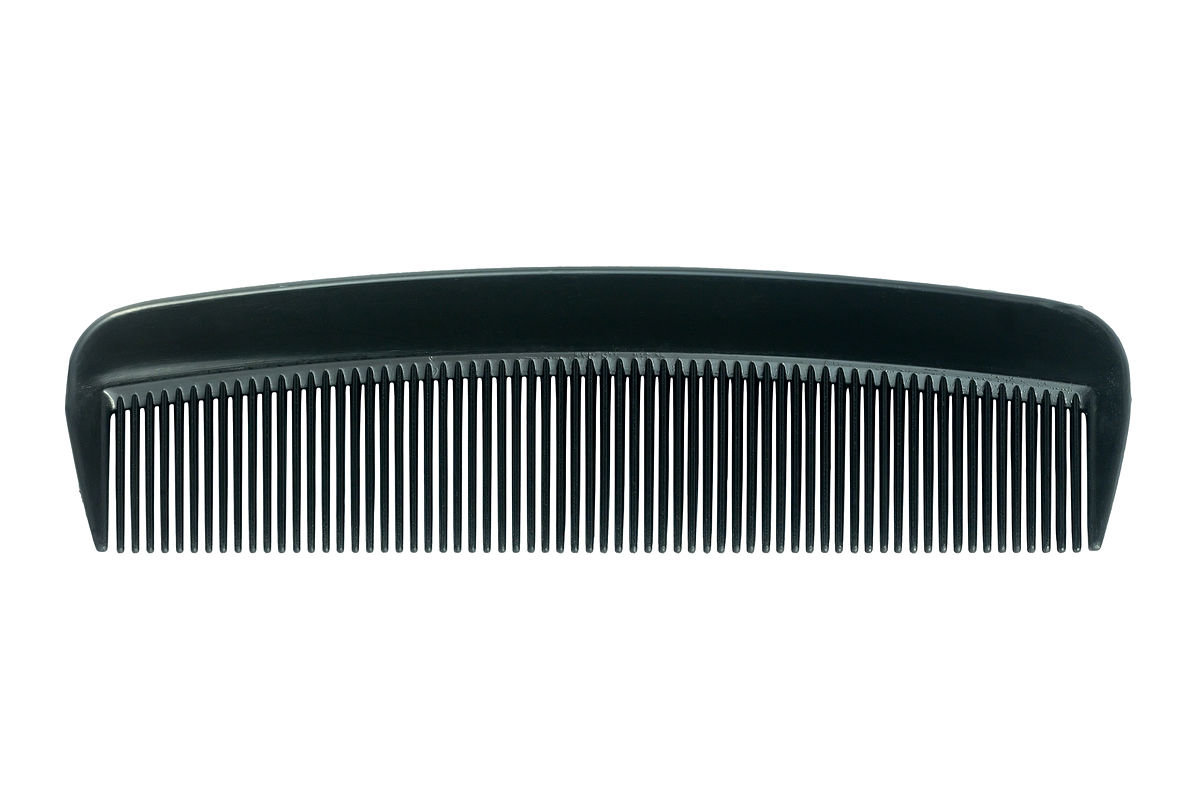
\includegraphics{images/comb.jpg}
\caption{comb.jpg}
\end{figure}

Psudocode of Hough:

\begin{figure}
\centering
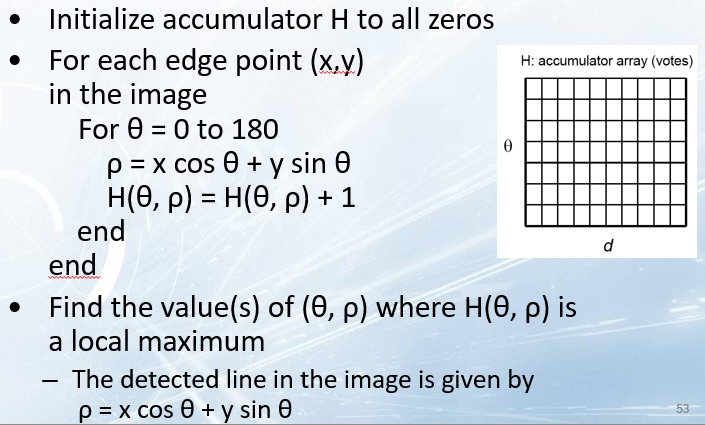
\includegraphics{wiki/psudo.jpg}
\caption{psudocode}
\end{figure}

    \hypertarget{a-hough-transformation-implementation}{%
\subsubsection{2.A Hough Transformation
Implementation}\label{a-hough-transformation-implementation}}

    \begin{Verbatim}[commandchars=\\\{\}]
{\color{incolor}In [{\color{incolor}254}]:} \PY{k}{def} \PY{n+nf}{show\PYZus{}hough\PYZus{}line}\PY{p}{(}\PY{n}{img}\PY{p}{,} \PY{n}{accumulator}\PY{p}{,} \PY{n}{thetas}\PY{p}{,} \PY{n}{rhos}\PY{p}{)}\PY{p}{:}
              \PY{n}{fig}\PY{p}{,} \PY{n}{ax} \PY{o}{=} \PY{n}{plt}\PY{o}{.}\PY{n}{subplots}\PY{p}{(}\PY{l+m+mi}{1}\PY{p}{,} \PY{l+m+mi}{2}\PY{p}{,} \PY{n}{figsize}\PY{o}{=}\PY{p}{(}\PY{l+m+mi}{15}\PY{p}{,} \PY{l+m+mi}{10}\PY{p}{)}\PY{p}{)}
          
              \PY{n}{ax}\PY{p}{[}\PY{l+m+mi}{0}\PY{p}{]}\PY{o}{.}\PY{n}{imshow}\PY{p}{(}\PY{n}{img}\PY{p}{,} \PY{n}{cmap}\PY{o}{=}\PY{l+s+s1}{\PYZsq{}}\PY{l+s+s1}{gray}\PY{l+s+s1}{\PYZsq{}}\PY{p}{)}
              \PY{n}{ax}\PY{p}{[}\PY{l+m+mi}{0}\PY{p}{]}\PY{o}{.}\PY{n}{set\PYZus{}title}\PY{p}{(}\PY{l+s+s1}{\PYZsq{}}\PY{l+s+s1}{Input image}\PY{l+s+s1}{\PYZsq{}}\PY{p}{)}
              \PY{n}{ax}\PY{p}{[}\PY{l+m+mi}{0}\PY{p}{]}\PY{o}{.}\PY{n}{axis}\PY{p}{(}\PY{l+s+s1}{\PYZsq{}}\PY{l+s+s1}{image}\PY{l+s+s1}{\PYZsq{}}\PY{p}{)}
          
              \PY{n}{ax}\PY{p}{[}\PY{l+m+mi}{1}\PY{p}{]}\PY{o}{.}\PY{n}{imshow}\PY{p}{(}\PY{n}{accumulator}\PY{p}{,} \PY{n}{cmap}\PY{o}{=}\PY{l+s+s1}{\PYZsq{}}\PY{l+s+s1}{gray}\PY{l+s+s1}{\PYZsq{}}\PY{p}{)}
              \PY{n}{ax}\PY{p}{[}\PY{l+m+mi}{1}\PY{p}{]}\PY{o}{.}\PY{n}{set\PYZus{}ylim}\PY{p}{(}\PY{o}{\PYZhy{}}\PY{l+m+mi}{90}\PY{p}{,} \PY{l+m+mi}{90}\PY{p}{)}
              \PY{n}{ax}\PY{p}{[}\PY{l+m+mi}{1}\PY{p}{]}\PY{o}{.}\PY{n}{set\PYZus{}title}\PY{p}{(}\PY{l+s+s1}{\PYZsq{}}\PY{l+s+s1}{Hough transform}\PY{l+s+s1}{\PYZsq{}}\PY{p}{)}
              \PY{n}{ax}\PY{p}{[}\PY{l+m+mi}{1}\PY{p}{]}\PY{o}{.}\PY{n}{set\PYZus{}xlabel}\PY{p}{(}\PY{l+s+s1}{\PYZsq{}}\PY{l+s+s1}{rho}\PY{l+s+s1}{\PYZsq{}}\PY{p}{)}
              \PY{n}{ax}\PY{p}{[}\PY{l+m+mi}{1}\PY{p}{]}\PY{o}{.}\PY{n}{set\PYZus{}ylabel}\PY{p}{(}\PY{l+s+s1}{\PYZsq{}}\PY{l+s+s1}{theta}\PY{l+s+s1}{\PYZsq{}}\PY{p}{)}
              \PY{n}{ax}\PY{p}{[}\PY{l+m+mi}{1}\PY{p}{]}\PY{o}{.}\PY{n}{axis}\PY{p}{(}\PY{l+s+s1}{\PYZsq{}}\PY{l+s+s1}{image}\PY{l+s+s1}{\PYZsq{}}\PY{p}{)}
\end{Verbatim}


    \begin{Verbatim}[commandchars=\\\{\}]
{\color{incolor}In [{\color{incolor}249}]:} \PY{k}{class} \PY{n+nc}{Gradient\PYZus{}Oriented\PYZus{}Hough}\PY{p}{:}
              \PY{l+s+sd}{\PYZdq{}\PYZdq{}\PYZdq{}}
          \PY{l+s+sd}{    Calculates the Hough transform of the input (grayscale) image with consideration of gradient magnitude}
          \PY{l+s+sd}{    \PYZdq{}\PYZdq{}\PYZdq{}}
              \PY{k}{def} \PY{n+nf}{\PYZus{}\PYZus{}init\PYZus{}\PYZus{}}\PY{p}{(}\PY{n+nb+bp}{self}\PY{p}{)}\PY{p}{:}
                  \PY{k}{pass}
              
              \PY{k}{def} \PY{n+nf}{\PYZus{}\PYZus{}call\PYZus{}\PYZus{}}\PY{p}{(}\PY{n+nb+bp}{self}\PY{p}{,} \PY{n}{image}\PY{p}{,} \PY{n}{delta\PYZus{}theta}\PY{p}{)}\PY{p}{:}
                  \PY{l+s+sd}{\PYZdq{}\PYZdq{}\PYZdq{}}
          \PY{l+s+sd}{        Gradient oriented Hough transform on grayscale image}
          \PY{l+s+sd}{        }
          \PY{l+s+sd}{        :param image: input image in form of ndarray or cv2 image}
          \PY{l+s+sd}{        :param delta\PYZus{}theta: Hypter\PYZhy{}parameter to control theta resolution of accumulator quantization}
          \PY{l+s+sd}{        :return: A tuple of (Accumulator, rhos, linear\PYZus{}theta, gradient\PYZus{}magnitude)}
          \PY{l+s+sd}{        \PYZdq{}\PYZdq{}\PYZdq{}}
                  \PY{c+c1}{\PYZsh{} Getting edges and gradient magnitude using Canny}
                  \PY{n}{image\PYZus{}grad}\PY{p}{,} \PY{n}{image\PYZus{}theta} \PY{o}{=} \PY{n}{GradientIntensity}\PY{p}{(}\PY{p}{)}\PY{p}{(}\PY{n}{GaussianNoise}\PY{p}{(}\PY{p}{)}\PY{p}{(}\PY{n}{image}\PY{p}{)}\PY{p}{)}
                  \PY{n}{edges} \PY{o}{=} \PY{n}{Thresholding}\PY{p}{(}\PY{p}{)}\PY{p}{(}\PY{n}{NonMaxSuppression}\PY{p}{(}\PY{p}{)}\PY{p}{(}\PY{n}{image\PYZus{}grad}\PY{p}{,} \PY{n}{image\PYZus{}theta}\PY{p}{)}\PY{p}{)}
                  \PY{n}{image\PYZus{}theta} \PY{o}{=} \PY{n}{np}\PY{o}{.}\PY{n}{array}\PY{p}{(}\PY{p}{[}\PY{n}{a}\PY{o}{\PYZpc{}}\PY{k}{180} for a in np.rad2deg(image\PYZus{}theta.flatten())]).reshape(image\PYZus{}grad.shape)
          
                  \PY{c+c1}{\PYZsh{} Gradient Oriented Hough}
                  \PY{n}{diag\PYZus{}len} \PY{o}{=} \PY{n}{np}\PY{o}{.}\PY{n}{uint64}\PY{p}{(}\PY{n}{np}\PY{o}{.}\PY{n}{ceil}\PY{p}{(}\PY{n}{np}\PY{o}{.}\PY{n}{hypot}\PY{p}{(}\PY{o}{*}\PY{n}{edges}\PY{o}{.}\PY{n}{shape}\PY{p}{)}\PY{p}{)}\PY{p}{)}
                  \PY{n}{rhos} \PY{o}{=} \PY{n}{np}\PY{o}{.}\PY{n}{linspace}\PY{p}{(}\PY{o}{\PYZhy{}}\PY{n}{diag\PYZus{}len}\PY{o}{/}\PY{l+m+mi}{2}\PY{p}{,} \PY{n}{diag\PYZus{}len}\PY{o}{/}\PY{l+m+mi}{2}\PY{p}{,} \PY{n}{diag\PYZus{}len}\PY{p}{)}
                  \PY{n}{for\PYZus{}good\PYZus{}measure} \PY{o}{=} \PY{l+m+mi}{15}  \PY{c+c1}{\PYZsh{} just to have a better visualization}
                  \PY{n}{accumulator} \PY{o}{=} \PY{n}{np}\PY{o}{.}\PY{n}{zeros}\PY{p}{(}\PY{p}{(}\PY{n+nb}{int}\PY{p}{(}\PY{n}{image\PYZus{}theta}\PY{o}{.}\PY{n}{max}\PY{p}{(}\PY{p}{)}\PY{o}{+}\PY{n}{for\PYZus{}good\PYZus{}measure}\PY{p}{)}\PY{p}{,} \PY{n+nb}{int}\PY{p}{(}\PY{n}{diag\PYZus{}len}\PY{p}{)}\PY{p}{)}\PY{p}{,} \PY{n}{dtype}\PY{o}{=}\PY{n}{np}\PY{o}{.}\PY{n}{int64}\PY{p}{)}
                  \PY{n}{x\PYZus{}edges}\PY{p}{,} \PY{n}{y\PYZus{}edges} \PY{o}{=} \PY{n}{np}\PY{o}{.}\PY{n}{where}\PY{p}{(}\PY{n}{edges}\PY{o}{==}\PY{l+m+mi}{255}\PY{p}{)}
                  \PY{k}{for} \PY{n}{idx} \PY{o+ow}{in} \PY{n+nb}{range}\PY{p}{(}\PY{n+nb}{len}\PY{p}{(}\PY{n}{x\PYZus{}edges}\PY{p}{)}\PY{p}{)}\PY{p}{:}
                      \PY{n}{x} \PY{o}{=} \PY{n}{x\PYZus{}edges}\PY{p}{[}\PY{n}{idx}\PY{p}{]}
                      \PY{n}{y} \PY{o}{=} \PY{n}{y\PYZus{}edges}\PY{p}{[}\PY{n}{idx}\PY{p}{]}
                      \PY{k}{if} \PY{n}{idx}\PY{o}{\PYZpc{}}\PY{k}{delta\PYZus{}theta} == 0:
                          \PY{n}{rho\PYZus{}} \PY{o}{=} \PY{n+nb}{int}\PY{p}{(}\PY{p}{(}\PY{n}{x}\PY{o}{*}\PY{n}{np}\PY{o}{.}\PY{n}{cos}\PY{p}{(}\PY{n}{image\PYZus{}theta}\PY{p}{[}\PY{n}{x}\PY{p}{,} \PY{n}{y}\PY{p}{]}\PY{p}{)} \PY{o}{+} \PY{n}{y}\PY{o}{*}\PY{n}{np}\PY{o}{.}\PY{n}{sin}\PY{p}{(}\PY{n}{image\PYZus{}theta}\PY{p}{[}\PY{n}{x}\PY{p}{,} \PY{n}{y}\PY{p}{]}\PY{p}{)}\PY{p}{)} \PY{o}{/} \PY{l+m+mi}{2}\PY{p}{)} \PY{o}{*} \PY{l+m+mi}{2}
                          \PY{n}{accumulator}\PY{p}{[}\PY{n+nb}{int}\PY{p}{(}\PY{n}{image\PYZus{}theta}\PY{p}{[}\PY{n}{x}\PY{p}{,} \PY{n}{y}\PY{p}{]}\PY{p}{)}\PY{p}{,} \PY{n}{rho\PYZus{}}\PY{p}{]} \PY{o}{+}\PY{o}{=} \PY{l+m+mi}{1}
                  \PY{k}{return} \PY{n}{accumulator}\PY{p}{,} \PY{n}{rhos}\PY{p}{,} \PY{n}{np}\PY{o}{.}\PY{n}{deg2rad}\PY{p}{(}\PY{n}{np}\PY{o}{.}\PY{n}{arange}\PY{p}{(}\PY{l+m+mi}{0}\PY{p}{,} \PY{n+nb}{int}\PY{p}{(}\PY{n}{image\PYZus{}theta}\PY{o}{.}\PY{n}{max}\PY{p}{(}\PY{p}{)}\PY{p}{)}\PY{p}{)}\PY{p}{)}\PY{p}{,} \PY{n}{image\PYZus{}theta}
          
          \PY{c+c1}{\PYZsh{} usage}
          \PY{n}{image} \PY{o}{=} \PY{n}{cv2}\PY{o}{.}\PY{n}{imread}\PY{p}{(}\PY{l+s+s1}{\PYZsq{}}\PY{l+s+s1}{images/comb.jpg}\PY{l+s+s1}{\PYZsq{}}\PY{p}{,} \PY{l+m+mi}{0}\PY{p}{)}\PY{o}{.}\PY{n}{astype}\PY{p}{(}\PY{n+nb}{float}\PY{p}{)}
          \PY{n}{accumulator}\PY{p}{,} \PY{n}{rhos}\PY{p}{,} \PY{n}{thetas}\PY{p}{,} \PY{n}{\PYZus{}} \PY{o}{=}  \PY{n}{Gradient\PYZus{}Oriented\PYZus{}Hough}\PY{p}{(}\PY{p}{)}\PY{p}{(}\PY{n}{image}\PY{p}{,} \PY{l+m+mi}{3}\PY{p}{)}
\end{Verbatim}


    \begin{Verbatim}[commandchars=\\\{\}]
{\color{incolor}In [{\color{incolor}245}]:} \PY{n}{show\PYZus{}hough\PYZus{}line}\PY{p}{(}\PY{n}{image}\PY{p}{,} \PY{n}{accumulator}\PY{p}{,} \PY{n}{thetas}\PY{p}{,} \PY{n}{rhos}\PY{p}{)}
\end{Verbatim}


    \begin{center}
    \adjustimage{max size={0.9\linewidth}{0.9\paperheight}}{output_31_0.png}
    \end{center}
    { \hspace*{\fill} \\}
    
    \begin{Verbatim}[commandchars=\\\{\}]
{\color{incolor}In [{\color{incolor}246}]:} \PY{k}{class} \PY{n+nc}{Hough}\PY{p}{:}
              \PY{l+s+sd}{\PYZdq{}\PYZdq{}\PYZdq{}}
          \PY{l+s+sd}{    Calculates Hough transform of a grayscale image}
          \PY{l+s+sd}{    \PYZdq{}\PYZdq{}\PYZdq{}}
              \PY{k}{def} \PY{n+nf}{\PYZus{}\PYZus{}init\PYZus{}\PYZus{}}\PY{p}{(}\PY{n+nb+bp}{self}\PY{p}{)}\PY{p}{:}
                  \PY{k}{pass}
              
              \PY{k}{def} \PY{n+nf}{\PYZus{}\PYZus{}call\PYZus{}\PYZus{}}\PY{p}{(}\PY{n+nb+bp}{self}\PY{p}{,} \PY{n}{image}\PY{p}{,} \PY{n}{theta\PYZus{}res}\PY{o}{=}\PY{l+m+mi}{90}\PY{p}{,} \PY{n}{delta\PYZus{}theta}\PY{o}{=}\PY{l+m+mi}{1}\PY{p}{)}\PY{p}{:}
                  \PY{l+s+sd}{\PYZdq{}\PYZdq{}\PYZdq{}}
          \PY{l+s+sd}{        Calculates Hough transform of input image using base algorithm}
          \PY{l+s+sd}{        }
          \PY{l+s+sd}{        :param image: input ndarray numpy image or cv2 image}
          \PY{l+s+sd}{        :param theta\PYZus{}res: Theta resolution which will be distributed between (\PYZhy{}theta\PYZus{}res, +theta\PYZus{}res) }
          \PY{l+s+sd}{        :param delta\PYZus{}theta: Hypter\PYZhy{}parameter to control theta resolution of accumulator quantization}
          \PY{l+s+sd}{        :return: A tuple of (Accumulator, rhos, thetas)}
          \PY{l+s+sd}{        \PYZdq{}\PYZdq{}\PYZdq{}}
                  \PY{c+c1}{\PYZsh{} Getting edges and gradient magnitude using Canny}
                  \PY{n}{image\PYZus{}grad}\PY{p}{,} \PY{n}{image\PYZus{}theta} \PY{o}{=} \PY{n}{GradientIntensity}\PY{p}{(}\PY{p}{)}\PY{p}{(}\PY{n}{GaussianNoise}\PY{p}{(}\PY{p}{)}\PY{p}{(}\PY{n}{image}\PY{p}{)}\PY{p}{)}
                  \PY{n}{edges} \PY{o}{=} \PY{n}{Thresholding}\PY{p}{(}\PY{p}{)}\PY{p}{(}\PY{n}{NonMaxSuppression}\PY{p}{(}\PY{p}{)}\PY{p}{(}\PY{n}{image\PYZus{}grad}\PY{p}{,} \PY{n}{image\PYZus{}theta}\PY{p}{)}\PY{p}{)}
          
                  \PY{c+c1}{\PYZsh{} Basic Hough}
                  \PY{n}{thetas} \PY{o}{=} \PY{n}{np}\PY{o}{.}\PY{n}{deg2rad}\PY{p}{(}\PY{n}{np}\PY{o}{.}\PY{n}{arange}\PY{p}{(}\PY{o}{\PYZhy{}}\PY{n}{theta\PYZus{}res}\PY{p}{,} \PY{n}{theta\PYZus{}res}\PY{p}{,} \PY{n}{delta\PYZus{}theta}\PY{p}{)}\PY{p}{)}
                  \PY{n}{diag\PYZus{}len} \PY{o}{=} \PY{n}{np}\PY{o}{.}\PY{n}{uint64}\PY{p}{(}\PY{n}{np}\PY{o}{.}\PY{n}{ceil}\PY{p}{(}\PY{n}{np}\PY{o}{.}\PY{n}{hypot}\PY{p}{(}\PY{o}{*}\PY{n}{edges}\PY{o}{.}\PY{n}{shape}\PY{p}{)}\PY{p}{)}\PY{p}{)}
                  \PY{n}{rhos} \PY{o}{=} \PY{n}{np}\PY{o}{.}\PY{n}{linspace}\PY{p}{(}\PY{o}{\PYZhy{}}\PY{n}{diag\PYZus{}len}\PY{o}{/}\PY{l+m+mi}{2}\PY{p}{,} \PY{n}{diag\PYZus{}len}\PY{o}{/}\PY{l+m+mi}{2}\PY{p}{,} \PY{n}{diag\PYZus{}len}\PY{p}{)}
                  \PY{n}{accumulator} \PY{o}{=} \PY{n}{np}\PY{o}{.}\PY{n}{zeros}\PY{p}{(}\PY{p}{(}\PY{n+nb}{len}\PY{p}{(}\PY{n}{thetas}\PY{p}{)}\PY{p}{,} \PY{n+nb}{int}\PY{p}{(}\PY{n}{diag\PYZus{}len}\PY{p}{)}\PY{p}{)}\PY{p}{,} \PY{n}{dtype}\PY{o}{=}\PY{n}{np}\PY{o}{.}\PY{n}{int64}\PY{p}{)}
                  \PY{n}{x\PYZus{}edges}\PY{p}{,} \PY{n}{y\PYZus{}edges} \PY{o}{=} \PY{n}{np}\PY{o}{.}\PY{n}{where}\PY{p}{(}\PY{n}{edges}\PY{o}{==}\PY{l+m+mi}{255}\PY{p}{)}
                  \PY{k}{for} \PY{n}{idx} \PY{o+ow}{in} \PY{n+nb}{range}\PY{p}{(}\PY{n+nb}{len}\PY{p}{(}\PY{n}{x\PYZus{}edges}\PY{p}{)}\PY{p}{)}\PY{p}{:}
                      \PY{k}{for} \PY{n}{j}\PY{p}{,} \PY{n}{t} \PY{o+ow}{in} \PY{n+nb}{enumerate}\PY{p}{(}\PY{n}{thetas}\PY{p}{)}\PY{p}{:}
                          \PY{n}{rho\PYZus{}} \PY{o}{=} \PY{n+nb}{int}\PY{p}{(}\PY{p}{(}\PY{n}{x\PYZus{}edges}\PY{p}{[}\PY{n}{idx}\PY{p}{]}\PY{o}{*}\PY{n}{np}\PY{o}{.}\PY{n}{cos}\PY{p}{(}\PY{n}{t}\PY{p}{)} \PY{o}{+} \PY{n}{y\PYZus{}edges}\PY{p}{[}\PY{n}{idx}\PY{p}{]}\PY{o}{*}\PY{n}{np}\PY{o}{.}\PY{n}{sin}\PY{p}{(}\PY{n}{t}\PY{p}{)}\PY{p}{)} \PY{o}{/} \PY{l+m+mi}{2}\PY{p}{)} \PY{o}{*} \PY{l+m+mi}{2}
                          \PY{n}{accumulator}\PY{p}{[}\PY{n}{j}\PY{p}{,} \PY{n}{rho\PYZus{}}\PY{p}{]} \PY{o}{+}\PY{o}{=} \PY{l+m+mi}{1}
                  \PY{k}{return} \PY{p}{(}\PY{n}{accumulator}\PY{p}{,} \PY{n}{rhos}\PY{p}{,} \PY{n}{thetas}\PY{p}{)}
          
          \PY{c+c1}{\PYZsh{} usage}
          \PY{n}{image} \PY{o}{=} \PY{n}{cv2}\PY{o}{.}\PY{n}{imread}\PY{p}{(}\PY{l+s+s1}{\PYZsq{}}\PY{l+s+s1}{images/comb.jpg}\PY{l+s+s1}{\PYZsq{}}\PY{p}{,} \PY{l+m+mi}{0}\PY{p}{)}\PY{o}{.}\PY{n}{astype}\PY{p}{(}\PY{n+nb}{float}\PY{p}{)}
          \PY{n}{accumulator}\PY{p}{,} \PY{n}{rhos}\PY{p}{,} \PY{n}{thetas} \PY{o}{=}  \PY{n}{Hough}\PY{p}{(}\PY{p}{)}\PY{p}{(}\PY{n}{image}\PY{p}{,} \PY{l+m+mi}{45}\PY{p}{,} \PY{l+m+mi}{2}\PY{p}{)}
\end{Verbatim}


    \begin{Verbatim}[commandchars=\\\{\}]
{\color{incolor}In [{\color{incolor}247}]:} \PY{n}{show\PYZus{}hough\PYZus{}line}\PY{p}{(}\PY{n}{image}\PY{p}{,} \PY{n}{accumulator}\PY{p}{,} \PY{n}{thetas}\PY{p}{,} \PY{n}{rhos}\PY{p}{)}
\end{Verbatim}


    \begin{center}
    \adjustimage{max size={0.9\linewidth}{0.9\paperheight}}{output_33_0.png}
    \end{center}
    { \hspace*{\fill} \\}
    
    \hypertarget{b-analyze-the-effect-of-delta_theta-on-gradient-oriented-hough}{%
\subsubsection{\texorpdfstring{2.B Analyze The Effect of
\texttt{delta\_theta} on Gradient Oriented
Hough}{2.B Analyze The Effect of delta\_theta on Gradient Oriented Hough}}\label{b-analyze-the-effect-of-delta_theta-on-gradient-oriented-hough}}

    \begin{Verbatim}[commandchars=\\\{\}]
{\color{incolor}In [{\color{incolor}263}]:} \PY{n}{image} \PY{o}{=} \PY{n}{cv2}\PY{o}{.}\PY{n}{imread}\PY{p}{(}\PY{l+s+s1}{\PYZsq{}}\PY{l+s+s1}{images/comb.jpg}\PY{l+s+s1}{\PYZsq{}}\PY{p}{,} \PY{l+m+mi}{0}\PY{p}{)}\PY{o}{.}\PY{n}{astype}\PY{p}{(}\PY{n+nb}{float}\PY{p}{)}
          \PY{n}{accumulator}\PY{p}{,} \PY{n}{rhos}\PY{p}{,} \PY{n}{thetas}\PY{p}{,} \PY{n}{\PYZus{}} \PY{o}{=}  \PY{n}{Gradient\PYZus{}Oriented\PYZus{}Hough}\PY{p}{(}\PY{p}{)}\PY{p}{(}\PY{n}{image}\PY{p}{,} \PY{l+m+mi}{1}\PY{p}{)}
          \PY{n}{show\PYZus{}hough\PYZus{}line}\PY{p}{(}\PY{n}{image}\PY{p}{,} \PY{n}{accumulator}\PY{p}{,} \PY{n}{thetas}\PY{p}{,} \PY{n}{rhos}\PY{p}{)}
\end{Verbatim}


    \begin{center}
    \adjustimage{max size={0.9\linewidth}{0.9\paperheight}}{output_35_0.png}
    \end{center}
    { \hspace*{\fill} \\}
    
    \begin{Verbatim}[commandchars=\\\{\}]
{\color{incolor}In [{\color{incolor}256}]:} \PY{n}{accumulator}\PY{p}{,} \PY{n}{rhos}\PY{p}{,} \PY{n}{thetas}\PY{p}{,} \PY{n}{\PYZus{}} \PY{o}{=}  \PY{n}{Gradient\PYZus{}Oriented\PYZus{}Hough}\PY{p}{(}\PY{p}{)}\PY{p}{(}\PY{n}{image}\PY{p}{,} \PY{l+m+mi}{5}\PY{p}{)}
          \PY{n}{show\PYZus{}hough\PYZus{}line}\PY{p}{(}\PY{n}{image}\PY{p}{,} \PY{n}{accumulator}\PY{p}{,} \PY{n}{thetas}\PY{p}{,} \PY{n}{rhos}\PY{p}{)}
\end{Verbatim}


    \begin{center}
    \adjustimage{max size={0.9\linewidth}{0.9\paperheight}}{output_36_0.png}
    \end{center}
    { \hspace*{\fill} \\}
    
    \begin{Verbatim}[commandchars=\\\{\}]
{\color{incolor}In [{\color{incolor}257}]:} \PY{n}{accumulator}\PY{p}{,} \PY{n}{rhos}\PY{p}{,} \PY{n}{thetas}\PY{p}{,} \PY{n}{\PYZus{}} \PY{o}{=}  \PY{n}{Gradient\PYZus{}Oriented\PYZus{}Hough}\PY{p}{(}\PY{p}{)}\PY{p}{(}\PY{n}{image}\PY{p}{,} \PY{l+m+mi}{15}\PY{p}{)}
          \PY{n}{show\PYZus{}hough\PYZus{}line}\PY{p}{(}\PY{n}{image}\PY{p}{,} \PY{n}{accumulator}\PY{p}{,} \PY{n}{thetas}\PY{p}{,} \PY{n}{rhos}\PY{p}{)}
\end{Verbatim}


    \begin{center}
    \adjustimage{max size={0.9\linewidth}{0.9\paperheight}}{output_37_0.png}
    \end{center}
    { \hspace*{\fill} \\}
    
    To compare these images, I have used following values: 1.
\texttt{delta\_theta\ =\ 1} for first image 2.
\texttt{delta\_theta\ =\ 5} for second image 3.
\texttt{delta\_theta\ =\ 15} for third image

For the first one, it has same resolution as the base image gradient
values so as we can see, there are lots of concentrated local maximas
that are indicating our lines. But when we increase
\texttt{delta\_theta} values in the follow-up images, the intensity of
concentrated areas decrease and in other areas of the transform, some
new local maxiams can be found and when we increase
\texttt{delta\_theta} further, some of previously detected lines will be
omitted and their votes will be shared by their neighbors or even
distributed over the space. The other point we can understand is that
when we increase the \texttt{delta\_theta} value, the accuracy decreases
but generalizations increases in contrary and it is less reliable as we
increase the value, because noises that previously has low votes and we
did not consider them as line, are contributing to the desired lines
which is not appropriate effect.

    \hypertarget{do-the-following-tasks-on-page.png-image}{%
\subsection{\texorpdfstring{3 Do the following tasks on
\texttt{page.png}
image:}{3 Do the following tasks on page.png image:}}\label{do-the-following-tasks-on-page.png-image}}

\begin{enumerate}
\def\labelenumi{\arabic{enumi}.}
\tightlist
\item
  Using \texttt{LineSegmentDetector} from \texttt{cv2}, extract the
  lines in the aforementioned image.
\item
  By using \textbf{line intersection}, find the four corners of the page
  and draw it.
\item
  Do the previous steps using \texttt{hough} transform from \texttt{cv2}
\item
  Compare results
\end{enumerate}

\begin{figure}
\centering
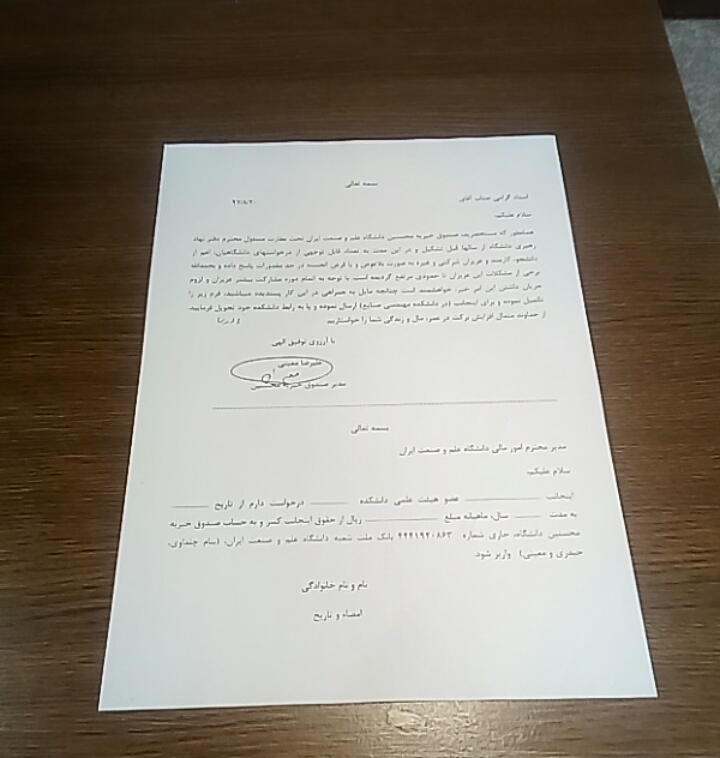
\includegraphics{images/page.png}
\caption{page.png}
\end{figure}

    \hypertarget{a-using-linesegmentdetector-from-cv2-extract-the-lines-of-the-image}{%
\subsubsection{\texorpdfstring{3.A Using \texttt{LineSegmentDetector}
From `cv2, Extract The Lines of The
image}{3.A Using LineSegmentDetector From `cv2, Extract The Lines of The image}}\label{a-using-linesegmentdetector-from-cv2-extract-the-lines-of-the-image}}

    \begin{Verbatim}[commandchars=\\\{\}]
{\color{incolor}In [{\color{incolor}578}]:} \PY{n}{image} \PY{o}{=} \PY{n}{cv2}\PY{o}{.}\PY{n}{imread}\PY{p}{(}\PY{l+s+s1}{\PYZsq{}}\PY{l+s+s1}{images/page.png}\PY{l+s+s1}{\PYZsq{}}\PY{p}{,} \PY{l+m+mi}{0}\PY{p}{)}
          \PY{n}{lsd} \PY{o}{=} \PY{n}{cv2}\PY{o}{.}\PY{n}{createLineSegmentDetector}\PY{p}{(}\PY{l+m+mi}{0}\PY{p}{)}
          \PY{n}{lines} \PY{o}{=} \PY{n}{lsd}\PY{o}{.}\PY{n}{detect}\PY{p}{(}\PY{n}{image}\PY{p}{)}\PY{p}{[}\PY{l+m+mi}{0}\PY{p}{]}
          \PY{n}{drawn\PYZus{}image} \PY{o}{=} \PY{n}{lsd}\PY{o}{.}\PY{n}{drawSegments}\PY{p}{(}\PY{n}{image}\PY{p}{,} \PY{n}{lines}\PY{p}{)}
          
          \PY{c+c1}{\PYZsh{} plotting}
          \PY{n}{plt}\PY{o}{.}\PY{n}{figure}\PY{p}{(}\PY{n}{figsize}\PY{o}{=}\PY{p}{(}\PY{l+m+mi}{20}\PY{p}{,}\PY{l+m+mi}{10}\PY{p}{)}\PY{p}{)}
          \PY{n}{plt}\PY{o}{.}\PY{n}{imshow}\PY{p}{(}\PY{n}{drawn\PYZus{}image}\PY{p}{)}
          \PY{n}{plt}\PY{o}{.}\PY{n}{show}\PY{p}{(}\PY{p}{)}
\end{Verbatim}


    \begin{center}
    \adjustimage{max size={0.9\linewidth}{0.9\paperheight}}{output_41_0.png}
    \end{center}
    { \hspace*{\fill} \\}
    
    \hypertarget{b-find-the-corners-using-linesegmentdetector}{%
\subsubsection{\texorpdfstring{3.B Find The Corners Using
\texttt{LineSegmentDetector}}{3.B Find The Corners Using LineSegmentDetector}}\label{b-find-the-corners-using-linesegmentdetector}}

The algorithm: 1. Extracting edges using available methods such as Canny
2. Segmenting image into background and target using flood fill
algorithms 3. Extracting edges using available methods such as Canny,
note that in this step, only the boundary of segmented areas exist 4.
Finding intersections

    \hypertarget{b.a-edge-extraction}{%
\paragraph{3.B.a Edge Extraction}\label{b.a-edge-extraction}}

    \begin{Verbatim}[commandchars=\\\{\}]
{\color{incolor}In [{\color{incolor}579}]:} \PY{n}{image} \PY{o}{=} \PY{n}{cv2}\PY{o}{.}\PY{n}{imread}\PY{p}{(}\PY{l+s+s1}{\PYZsq{}}\PY{l+s+s1}{images/page.png}\PY{l+s+s1}{\PYZsq{}}\PY{p}{,} \PY{l+m+mi}{0}\PY{p}{)}
          \PY{n}{edges} \PY{o}{=} \PY{n}{cv2}\PY{o}{.}\PY{n}{Canny}\PY{p}{(}\PY{n}{image}\PY{p}{,} \PY{l+m+mi}{150}\PY{p}{,} \PY{l+m+mi}{200}\PY{p}{)}
          \PY{n}{plt}\PY{o}{.}\PY{n}{imshow}\PY{p}{(}\PY{n}{edges}\PY{p}{,} \PY{n}{cmap}\PY{o}{=}\PY{l+s+s1}{\PYZsq{}}\PY{l+s+s1}{gray}\PY{l+s+s1}{\PYZsq{}}\PY{p}{)}
\end{Verbatim}


\begin{Verbatim}[commandchars=\\\{\}]
{\color{outcolor}Out[{\color{outcolor}579}]:} <matplotlib.image.AxesImage at 0x25002f0beb8>
\end{Verbatim}
            
    \begin{center}
    \adjustimage{max size={0.9\linewidth}{0.9\paperheight}}{output_44_1.png}
    \end{center}
    { \hspace*{\fill} \\}
    
    \hypertarget{b.b-image-segmentation}{%
\paragraph{3.B.b Image Segmentation}\label{b.b-image-segmentation}}

    \begin{Verbatim}[commandchars=\\\{\}]
{\color{incolor}In [{\color{incolor}580}]:} \PY{n}{mask} \PY{o}{=} \PY{n}{np}\PY{o}{.}\PY{n}{zeros}\PY{p}{(}\PY{p}{(}\PY{n}{image}\PY{o}{.}\PY{n}{shape}\PY{p}{[}\PY{l+m+mi}{0}\PY{p}{]}\PY{o}{+}\PY{l+m+mi}{2}\PY{p}{,} \PY{n}{image}\PY{o}{.}\PY{n}{shape}\PY{p}{[}\PY{l+m+mi}{1}\PY{p}{]}\PY{o}{+}\PY{l+m+mi}{2}\PY{p}{)}\PY{p}{,} \PY{n}{np}\PY{o}{.}\PY{n}{uint8}\PY{p}{)}
          \PY{n}{arbitrary} \PY{o}{=} \PY{l+m+mi}{150}  \PY{c+c1}{\PYZsh{} any value except 255 because edges are 255}
          \PY{n}{flooded} \PY{o}{=} \PY{n}{cv2}\PY{o}{.}\PY{n}{floodFill}\PY{p}{(}\PY{n}{edges}\PY{p}{,} \PY{n}{mask}\PY{p}{,} \PY{p}{(}\PY{l+m+mi}{0}\PY{p}{,}\PY{l+m+mi}{0}\PY{p}{)}\PY{p}{,} \PY{n}{arbitrary}\PY{p}{)}\PY{p}{[}\PY{l+m+mi}{1}\PY{p}{]}
          \PY{n}{plt}\PY{o}{.}\PY{n}{imshow}\PY{p}{(}\PY{n}{flooded}\PY{p}{,} \PY{n}{cmap}\PY{o}{=}\PY{l+s+s1}{\PYZsq{}}\PY{l+s+s1}{gray}\PY{l+s+s1}{\PYZsq{}}\PY{p}{)}
\end{Verbatim}


\begin{Verbatim}[commandchars=\\\{\}]
{\color{outcolor}Out[{\color{outcolor}580}]:} <matplotlib.image.AxesImage at 0x25004abd438>
\end{Verbatim}
            
    \begin{center}
    \adjustimage{max size={0.9\linewidth}{0.9\paperheight}}{output_46_1.png}
    \end{center}
    { \hspace*{\fill} \\}
    
    \begin{Verbatim}[commandchars=\\\{\}]
{\color{incolor}In [{\color{incolor}581}]:} \PY{n}{flooded\PYZus{}mask} \PY{o}{=} \PY{n}{np}\PY{o}{.}\PY{n}{zeros}\PY{p}{(}\PY{p}{(}\PY{n}{flooded}\PY{o}{.}\PY{n}{shape}\PY{p}{)}\PY{p}{)}
          \PY{n}{flooded\PYZus{}mask}\PY{p}{[}\PY{n}{edges} \PY{o}{==} \PY{n}{arbitrary}\PY{p}{]} \PY{o}{=} \PY{l+m+mi}{255}
          \PY{n}{plt}\PY{o}{.}\PY{n}{imshow}\PY{p}{(}\PY{n}{flooded\PYZus{}mask}\PY{p}{,} \PY{n}{cmap}\PY{o}{=}\PY{l+s+s1}{\PYZsq{}}\PY{l+s+s1}{gray}\PY{l+s+s1}{\PYZsq{}}\PY{p}{)}
\end{Verbatim}


\begin{Verbatim}[commandchars=\\\{\}]
{\color{outcolor}Out[{\color{outcolor}581}]:} <matplotlib.image.AxesImage at 0x25004b0aeb8>
\end{Verbatim}
            
    \begin{center}
    \adjustimage{max size={0.9\linewidth}{0.9\paperheight}}{output_47_1.png}
    \end{center}
    { \hspace*{\fill} \\}
    
    \hypertarget{b.c-edge-extraction-of-segmented-areas}{%
\paragraph{3.B.c Edge Extraction of Segmented
Areas}\label{b.c-edge-extraction-of-segmented-areas}}

    \begin{Verbatim}[commandchars=\\\{\}]
{\color{incolor}In [{\color{incolor}583}]:} \PY{n}{segmented\PYZus{}edges} \PY{o}{=} \PY{n}{cv2}\PY{o}{.}\PY{n}{Canny}\PY{p}{(}\PY{n}{np}\PY{o}{.}\PY{n}{uint8}\PY{p}{(}\PY{n}{flooded\PYZus{}mask}\PY{p}{)}\PY{p}{,} \PY{l+m+mi}{100}\PY{p}{,} \PY{l+m+mi}{200}\PY{p}{,} \PY{n}{L2gradient}\PY{o}{=}\PY{k+kc}{True}\PY{p}{)}
          \PY{n}{plt}\PY{o}{.}\PY{n}{imshow}\PY{p}{(}\PY{n}{segmented\PYZus{}edges}\PY{p}{,} \PY{n}{cmap}\PY{o}{=}\PY{l+s+s1}{\PYZsq{}}\PY{l+s+s1}{gray}\PY{l+s+s1}{\PYZsq{}}\PY{p}{)}
\end{Verbatim}


\begin{Verbatim}[commandchars=\\\{\}]
{\color{outcolor}Out[{\color{outcolor}583}]:} <matplotlib.image.AxesImage at 0x250051bbeb8>
\end{Verbatim}
            
    \begin{center}
    \adjustimage{max size={0.9\linewidth}{0.9\paperheight}}{output_49_1.png}
    \end{center}
    { \hspace*{\fill} \\}
    
    \begin{Verbatim}[commandchars=\\\{\}]
{\color{incolor}In [{\color{incolor}584}]:} \PY{n}{lsd} \PY{o}{=} \PY{n}{cv2}\PY{o}{.}\PY{n}{createLineSegmentDetector}\PY{p}{(}\PY{l+m+mi}{0}\PY{p}{)}
          \PY{n}{plane\PYZus{}} \PY{o}{=} \PY{n}{np}\PY{o}{.}\PY{n}{zeros}\PY{p}{(}\PY{p}{(}\PY{n}{segmented\PYZus{}edges}\PY{o}{.}\PY{n}{shape}\PY{p}{)}\PY{p}{)}
          \PY{n}{lines} \PY{o}{=} \PY{n}{lsd}\PY{o}{.}\PY{n}{detect}\PY{p}{(}\PY{n}{segmented\PYZus{}edges}\PY{o}{.}\PY{n}{astype}\PY{p}{(}\PY{l+s+s1}{\PYZsq{}}\PY{l+s+s1}{uint8}\PY{l+s+s1}{\PYZsq{}}\PY{p}{)}\PY{p}{)}\PY{p}{[}\PY{l+m+mi}{0}\PY{p}{]}
          \PY{n}{drawn\PYZus{}image} \PY{o}{=} \PY{n}{lsd}\PY{o}{.}\PY{n}{drawSegments}\PY{p}{(}\PY{n}{plane\PYZus{}}\PY{p}{,} \PY{n}{lines}\PY{p}{)}
          
          \PY{c+c1}{\PYZsh{} plotting}
          \PY{n}{plt}\PY{o}{.}\PY{n}{imshow}\PY{p}{(}\PY{n}{drawn\PYZus{}image}\PY{p}{)}
          \PY{n}{plt}\PY{o}{.}\PY{n}{show}\PY{p}{(}\PY{p}{)}
\end{Verbatim}


    \begin{Verbatim}[commandchars=\\\{\}]
Clipping input data to the valid range for imshow with RGB data ([0..1] for floats or [0..255] for integers).

    \end{Verbatim}

    \begin{center}
    \adjustimage{max size={0.9\linewidth}{0.9\paperheight}}{output_50_1.png}
    \end{center}
    { \hspace*{\fill} \\}
    
    \begin{Verbatim}[commandchars=\\\{\}]
{\color{incolor}In [{\color{incolor}585}]:} \PY{k}{for} \PY{n}{l} \PY{o+ow}{in} \PY{n+nb}{range}\PY{p}{(}\PY{n+nb}{len}\PY{p}{(}\PY{n}{lines}\PY{p}{)}\PY{p}{)}\PY{p}{:}
              \PY{n}{xy} \PY{o}{=} \PY{n}{line\PYZus{}intersection}\PY{p}{(}\PY{n}{lines}\PY{p}{[}\PY{n}{l}\PY{p}{]}\PY{p}{,} \PY{n}{lines}\PY{p}{[}\PY{n}{l}\PY{o}{\PYZhy{}}\PY{l+m+mi}{1}\PY{p}{]}\PY{p}{,} \PY{k+kc}{False}\PY{p}{)}
              \PY{k}{if} \PY{n}{xy}\PY{p}{[}\PY{l+m+mi}{0}\PY{p}{]}\PY{o}{\PYZlt{}}\PY{l+m+mi}{0} \PY{o+ow}{or} \PY{n}{xy}\PY{p}{[}\PY{l+m+mi}{1}\PY{p}{]}\PY{o}{\PYZlt{}}\PY{l+m+mi}{0} \PY{o+ow}{or} \PY{n}{xy}\PY{p}{[}\PY{l+m+mi}{0}\PY{p}{]}\PY{o}{\PYZgt{}}\PY{n}{plane}\PY{o}{.}\PY{n}{shape}\PY{p}{[}\PY{l+m+mi}{0}\PY{p}{]} \PY{o+ow}{or} \PY{n}{xy}\PY{p}{[}\PY{l+m+mi}{1}\PY{p}{]}\PY{o}{\PYZgt{}}\PY{n}{plane\PYZus{}}\PY{o}{.}\PY{n}{shape}\PY{p}{[}\PY{l+m+mi}{1}\PY{p}{]}\PY{p}{:}
                  \PY{k}{continue}
          \PY{c+c1}{\PYZsh{}     print(xy)}
              \PY{n}{plane\PYZus{}} \PY{o}{=} \PY{n}{cv2}\PY{o}{.}\PY{n}{circle}\PY{p}{(}\PY{n}{drawn\PYZus{}image}\PY{p}{,} \PY{n}{xy}\PY{p}{,} \PY{l+m+mi}{5}\PY{p}{,} \PY{l+m+mi}{255}\PY{p}{,} \PY{l+m+mi}{2}\PY{p}{)}
          \PY{n}{plt}\PY{o}{.}\PY{n}{imshow}\PY{p}{(}\PY{n}{plane\PYZus{}}\PY{p}{)}
\end{Verbatim}


    \begin{Verbatim}[commandchars=\\\{\}]
Clipping input data to the valid range for imshow with RGB data ([0..1] for floats or [0..255] for integers).

    \end{Verbatim}

\begin{Verbatim}[commandchars=\\\{\}]
{\color{outcolor}Out[{\color{outcolor}585}]:} <matplotlib.image.AxesImage at 0x2500500ca20>
\end{Verbatim}
            
    \begin{center}
    \adjustimage{max size={0.9\linewidth}{0.9\paperheight}}{output_51_2.png}
    \end{center}
    { \hspace*{\fill} \\}
    
    \begin{Verbatim}[commandchars=\\\{\}]
{\color{incolor}In [{\color{incolor}586}]:} \PY{k}{def} \PY{n+nf}{line\PYZus{}intersection}\PY{p}{(}\PY{n}{line1}\PY{p}{,} \PY{n}{line2}\PY{p}{,} \PY{n}{polar}\PY{o}{=}\PY{k+kc}{False}\PY{p}{)}\PY{p}{:}
              \PY{k}{if} \PY{o+ow}{not} \PY{n}{polar}\PY{p}{:}
                  \PY{n}{line1} \PY{o}{=} \PY{n}{line1}\PY{o}{.}\PY{n}{reshape}\PY{p}{(}\PY{l+m+mi}{2}\PY{p}{,} \PY{l+m+mi}{2}\PY{p}{)}
                  \PY{n}{line2} \PY{o}{=} \PY{n}{line2}\PY{o}{.}\PY{n}{reshape}\PY{p}{(}\PY{l+m+mi}{2}\PY{p}{,} \PY{l+m+mi}{2}\PY{p}{)}
                  \PY{n}{xdiff} \PY{o}{=} \PY{p}{(}\PY{n}{line1}\PY{p}{[}\PY{l+m+mi}{0}\PY{p}{]}\PY{p}{[}\PY{l+m+mi}{0}\PY{p}{]} \PY{o}{\PYZhy{}} \PY{n}{line1}\PY{p}{[}\PY{l+m+mi}{1}\PY{p}{]}\PY{p}{[}\PY{l+m+mi}{0}\PY{p}{]}\PY{p}{,} \PY{n}{line2}\PY{p}{[}\PY{l+m+mi}{0}\PY{p}{]}\PY{p}{[}\PY{l+m+mi}{0}\PY{p}{]} \PY{o}{\PYZhy{}} \PY{n}{line2}\PY{p}{[}\PY{l+m+mi}{1}\PY{p}{]}\PY{p}{[}\PY{l+m+mi}{0}\PY{p}{]}\PY{p}{)}
                  \PY{n}{ydiff} \PY{o}{=} \PY{p}{(}\PY{n}{line1}\PY{p}{[}\PY{l+m+mi}{0}\PY{p}{]}\PY{p}{[}\PY{l+m+mi}{1}\PY{p}{]} \PY{o}{\PYZhy{}} \PY{n}{line1}\PY{p}{[}\PY{l+m+mi}{1}\PY{p}{]}\PY{p}{[}\PY{l+m+mi}{1}\PY{p}{]}\PY{p}{,} \PY{n}{line2}\PY{p}{[}\PY{l+m+mi}{0}\PY{p}{]}\PY{p}{[}\PY{l+m+mi}{1}\PY{p}{]} \PY{o}{\PYZhy{}} \PY{n}{line2}\PY{p}{[}\PY{l+m+mi}{1}\PY{p}{]}\PY{p}{[}\PY{l+m+mi}{1}\PY{p}{]}\PY{p}{)}
          
                  \PY{k}{def} \PY{n+nf}{det}\PY{p}{(}\PY{n}{a}\PY{p}{,} \PY{n}{b}\PY{p}{)}\PY{p}{:}
                      \PY{k}{return} \PY{n}{a}\PY{p}{[}\PY{l+m+mi}{0}\PY{p}{]} \PY{o}{*} \PY{n}{b}\PY{p}{[}\PY{l+m+mi}{1}\PY{p}{]} \PY{o}{\PYZhy{}} \PY{n}{a}\PY{p}{[}\PY{l+m+mi}{1}\PY{p}{]} \PY{o}{*} \PY{n}{b}\PY{p}{[}\PY{l+m+mi}{0}\PY{p}{]}
          
                  \PY{n}{div} \PY{o}{=} \PY{n}{det}\PY{p}{(}\PY{n}{xdiff}\PY{p}{,} \PY{n}{ydiff}\PY{p}{)}
                  \PY{k}{if} \PY{n}{div} \PY{o}{==} \PY{l+m+mi}{0}\PY{p}{:}
                     \PY{k}{return} \PY{o}{\PYZhy{}}\PY{l+m+mi}{1}\PY{p}{,} \PY{o}{\PYZhy{}}\PY{l+m+mi}{1}
                  \PY{n}{d} \PY{o}{=} \PY{p}{(}\PY{n}{det}\PY{p}{(}\PY{o}{*}\PY{n}{line1}\PY{p}{)}\PY{p}{,} \PY{n}{det}\PY{p}{(}\PY{o}{*}\PY{n}{line2}\PY{p}{)}\PY{p}{)}
                  \PY{n}{x} \PY{o}{=} \PY{n}{det}\PY{p}{(}\PY{n}{d}\PY{p}{,} \PY{n}{xdiff}\PY{p}{)} \PY{o}{/} \PY{n}{div}
                  \PY{n}{y} \PY{o}{=} \PY{n}{det}\PY{p}{(}\PY{n}{d}\PY{p}{,} \PY{n}{ydiff}\PY{p}{)} \PY{o}{/} \PY{n}{div}
                  \PY{k}{return} \PY{n}{x}\PY{p}{,} \PY{n}{y}
              \PY{k}{else}\PY{p}{:}
                  \PY{n}{rho1}\PY{p}{,} \PY{n}{theta1} \PY{o}{=} \PY{n}{line1}\PY{p}{[}\PY{l+m+mi}{0}\PY{p}{]}
                  \PY{n}{rho2}\PY{p}{,} \PY{n}{theta2} \PY{o}{=} \PY{n}{line2}\PY{p}{[}\PY{l+m+mi}{0}\PY{p}{]}
                  \PY{n}{A} \PY{o}{=} \PY{n}{np}\PY{o}{.}\PY{n}{array}\PY{p}{(}\PY{p}{[}
                      \PY{p}{[}\PY{n}{np}\PY{o}{.}\PY{n}{cos}\PY{p}{(}\PY{n}{theta1}\PY{p}{)}\PY{p}{,} \PY{n}{np}\PY{o}{.}\PY{n}{sin}\PY{p}{(}\PY{n}{theta1}\PY{p}{)}\PY{p}{]}\PY{p}{,}
                      \PY{p}{[}\PY{n}{np}\PY{o}{.}\PY{n}{cos}\PY{p}{(}\PY{n}{theta2}\PY{p}{)}\PY{p}{,} \PY{n}{np}\PY{o}{.}\PY{n}{sin}\PY{p}{(}\PY{n}{theta2}\PY{p}{)}\PY{p}{]}
                  \PY{p}{]}\PY{p}{)}
                  \PY{n}{b} \PY{o}{=} \PY{n}{np}\PY{o}{.}\PY{n}{array}\PY{p}{(}\PY{p}{[}\PY{p}{[}\PY{n}{rho1}\PY{p}{]}\PY{p}{,} \PY{p}{[}\PY{n}{rho2}\PY{p}{]}\PY{p}{]}\PY{p}{)}
                  \PY{k}{try}\PY{p}{:}
                      \PY{n}{x0}\PY{p}{,} \PY{n}{y0} \PY{o}{=} \PY{n}{np}\PY{o}{.}\PY{n}{linalg}\PY{o}{.}\PY{n}{solve}\PY{p}{(}\PY{n}{A}\PY{p}{,} \PY{n}{b}\PY{p}{)}
                  \PY{k}{except}\PY{p}{:}
                      \PY{k}{return} \PY{p}{[}\PY{o}{\PYZhy{}}\PY{l+m+mi}{1}\PY{p}{,} \PY{o}{\PYZhy{}}\PY{l+m+mi}{1}\PY{p}{]}
                  \PY{n}{x0}\PY{p}{,} \PY{n}{y0} \PY{o}{=} \PY{n+nb}{int}\PY{p}{(}\PY{n}{np}\PY{o}{.}\PY{n}{round}\PY{p}{(}\PY{n}{x0}\PY{p}{)}\PY{p}{)}\PY{p}{,} \PY{n+nb}{int}\PY{p}{(}\PY{n}{np}\PY{o}{.}\PY{n}{round}\PY{p}{(}\PY{n}{y0}\PY{p}{)}\PY{p}{)}
                  \PY{k}{return} \PY{p}{[}\PY{n}{x0}\PY{p}{,} \PY{n}{y0}\PY{p}{]}
              
\end{Verbatim}


    \hypertarget{c-find-the-corners-using-houghlines}{%
\subsubsection{\texorpdfstring{3.C Find The Corners Using
\texttt{HoughLines}}{3.C Find The Corners Using HoughLines}}\label{c-find-the-corners-using-houghlines}}

    \begin{Verbatim}[commandchars=\\\{\}]
{\color{incolor}In [{\color{incolor}587}]:} \PY{n}{image} \PY{o}{=} \PY{n}{cv2}\PY{o}{.}\PY{n}{imread}\PY{p}{(}\PY{l+s+s1}{\PYZsq{}}\PY{l+s+s1}{images/page.png}\PY{l+s+s1}{\PYZsq{}}\PY{p}{,} \PY{l+m+mi}{0}\PY{p}{)}
          \PY{n}{plane} \PY{o}{=} \PY{n}{np}\PY{o}{.}\PY{n}{zeros}\PY{p}{(}\PY{n}{image}\PY{o}{.}\PY{n}{shape}\PY{p}{)}
          \PY{n}{lines} \PY{o}{=} \PY{n}{cv2}\PY{o}{.}\PY{n}{HoughLines}\PY{p}{(}\PY{n}{segmented\PYZus{}edges}\PY{p}{,} \PY{l+m+mf}{0.77}\PY{p}{,} \PY{n}{np}\PY{o}{.}\PY{n}{pi} \PY{o}{/} \PY{l+m+mi}{183}\PY{p}{,} \PY{l+m+mi}{100}\PY{p}{,} \PY{k+kc}{None}\PY{p}{,} \PY{l+m+mi}{0}\PY{p}{,} \PY{l+m+mi}{0}\PY{p}{)}  \PY{c+c1}{\PYZsh{} hyper\PYZhy{}parameter tuned using grid search then manually!}
          \PY{c+c1}{\PYZsh{} Draw the lines}
          \PY{k}{if} \PY{n}{lines} \PY{o+ow}{is} \PY{o+ow}{not} \PY{k+kc}{None}\PY{p}{:}
              \PY{k}{for} \PY{n}{i} \PY{o+ow}{in} \PY{n+nb}{range}\PY{p}{(}\PY{n+nb}{len}\PY{p}{(}\PY{n}{lines}\PY{p}{)}\PY{p}{)}\PY{p}{:}
                  \PY{n}{rho} \PY{o}{=} \PY{n}{lines}\PY{p}{[}\PY{n}{i}\PY{p}{]}\PY{p}{[}\PY{l+m+mi}{0}\PY{p}{]}\PY{p}{[}\PY{l+m+mi}{0}\PY{p}{]}
                  \PY{n}{theta} \PY{o}{=} \PY{n}{lines}\PY{p}{[}\PY{n}{i}\PY{p}{]}\PY{p}{[}\PY{l+m+mi}{0}\PY{p}{]}\PY{p}{[}\PY{l+m+mi}{1}\PY{p}{]}
                  \PY{n}{a} \PY{o}{=} \PY{n}{np}\PY{o}{.}\PY{n}{cos}\PY{p}{(}\PY{n}{theta}\PY{p}{)}
                  \PY{n}{b} \PY{o}{=} \PY{n}{np}\PY{o}{.}\PY{n}{sin}\PY{p}{(}\PY{n}{theta}\PY{p}{)}
                  \PY{n}{x0} \PY{o}{=} \PY{n}{a} \PY{o}{*} \PY{n}{rho}
                  \PY{n}{y0} \PY{o}{=} \PY{n}{b} \PY{o}{*} \PY{n}{rho}
                  \PY{n}{pt1} \PY{o}{=} \PY{p}{(}\PY{n+nb}{int}\PY{p}{(}\PY{n}{x0} \PY{o}{+} \PY{l+m+mi}{1000}\PY{o}{*}\PY{p}{(}\PY{o}{\PYZhy{}}\PY{n}{b}\PY{p}{)}\PY{p}{)}\PY{p}{,} \PY{n+nb}{int}\PY{p}{(}\PY{n}{y0} \PY{o}{+} \PY{l+m+mi}{1000}\PY{o}{*}\PY{p}{(}\PY{n}{a}\PY{p}{)}\PY{p}{)}\PY{p}{)}
                  \PY{n}{pt2} \PY{o}{=} \PY{p}{(}\PY{n+nb}{int}\PY{p}{(}\PY{n}{x0} \PY{o}{\PYZhy{}} \PY{l+m+mi}{1000}\PY{o}{*}\PY{p}{(}\PY{o}{\PYZhy{}}\PY{n}{b}\PY{p}{)}\PY{p}{)}\PY{p}{,} \PY{n+nb}{int}\PY{p}{(}\PY{n}{y0} \PY{o}{\PYZhy{}} \PY{l+m+mi}{1000}\PY{o}{*}\PY{p}{(}\PY{n}{a}\PY{p}{)}\PY{p}{)}\PY{p}{)}
                  \PY{n}{cv2}\PY{o}{.}\PY{n}{line}\PY{p}{(}\PY{n}{plane}\PY{p}{,} \PY{n}{pt1}\PY{p}{,} \PY{n}{pt2}\PY{p}{,} \PY{p}{(}\PY{n}{arbitrary}\PY{p}{,} \PY{l+m+mi}{234}\PY{p}{,} \PY{n}{arbitrary}\PY{p}{)}\PY{p}{,} \PY{l+m+mi}{2}\PY{p}{,} \PY{n}{cv2}\PY{o}{.}\PY{n}{LINE\PYZus{}AA}\PY{p}{)}
          \PY{n}{plt}\PY{o}{.}\PY{n}{imshow}\PY{p}{(}\PY{n}{plane}\PY{p}{,} \PY{n}{cmap}\PY{o}{=}\PY{l+s+s1}{\PYZsq{}}\PY{l+s+s1}{jet}\PY{l+s+s1}{\PYZsq{}}\PY{p}{)}
\end{Verbatim}


\begin{Verbatim}[commandchars=\\\{\}]
{\color{outcolor}Out[{\color{outcolor}587}]:} <matplotlib.image.AxesImage at 0x25004b86b38>
\end{Verbatim}
            
    \begin{center}
    \adjustimage{max size={0.9\linewidth}{0.9\paperheight}}{output_54_1.png}
    \end{center}
    { \hspace*{\fill} \\}
    
    \begin{Verbatim}[commandchars=\\\{\}]
{\color{incolor}In [{\color{incolor}588}]:} \PY{k}{for} \PY{n}{l} \PY{o+ow}{in} \PY{n+nb}{range}\PY{p}{(}\PY{n+nb}{len}\PY{p}{(}\PY{n}{lines}\PY{p}{)}\PY{p}{)}\PY{p}{:}
              \PY{n}{xy} \PY{o}{=} \PY{n+nb}{tuple}\PY{p}{(}\PY{n}{line\PYZus{}intersection}\PY{p}{(}\PY{n}{lines}\PY{p}{[}\PY{n}{l}\PY{p}{]}\PY{p}{,} \PY{n}{lines}\PY{p}{[}\PY{n}{l}\PY{o}{\PYZhy{}}\PY{l+m+mi}{1}\PY{p}{]}\PY{p}{,} \PY{n}{polar}\PY{o}{=}\PY{k+kc}{True}\PY{p}{)}\PY{p}{)}
              \PY{k}{if} \PY{n}{xy}\PY{p}{[}\PY{l+m+mi}{0}\PY{p}{]}\PY{o}{\PYZlt{}}\PY{l+m+mi}{0} \PY{o+ow}{or} \PY{n}{xy}\PY{p}{[}\PY{l+m+mi}{1}\PY{p}{]}\PY{o}{\PYZlt{}}\PY{l+m+mi}{0} \PY{o+ow}{or} \PY{n}{xy}\PY{p}{[}\PY{l+m+mi}{0}\PY{p}{]}\PY{o}{\PYZgt{}}\PY{n}{plane}\PY{o}{.}\PY{n}{shape}\PY{p}{[}\PY{l+m+mi}{0}\PY{p}{]} \PY{o+ow}{or} \PY{n}{xy}\PY{p}{[}\PY{l+m+mi}{1}\PY{p}{]}\PY{o}{\PYZgt{}}\PY{n}{plane}\PY{o}{.}\PY{n}{shape}\PY{p}{[}\PY{l+m+mi}{1}\PY{p}{]}\PY{p}{:}
                  \PY{k}{continue}
              \PY{n}{plane} \PY{o}{=} \PY{n}{cv2}\PY{o}{.}\PY{n}{circle}\PY{p}{(}\PY{n}{plane}\PY{p}{,} \PY{n}{xy}\PY{p}{,} \PY{l+m+mi}{10}\PY{p}{,} \PY{l+m+mi}{255}\PY{p}{,} \PY{l+m+mi}{2}\PY{p}{)}
          \PY{n}{plt}\PY{o}{.}\PY{n}{imshow}\PY{p}{(}\PY{n}{plane}\PY{p}{)}
\end{Verbatim}


\begin{Verbatim}[commandchars=\\\{\}]
{\color{outcolor}Out[{\color{outcolor}588}]:} <matplotlib.image.AxesImage at 0x25004bdbba8>
\end{Verbatim}
            
    \begin{center}
    \adjustimage{max size={0.9\linewidth}{0.9\paperheight}}{output_55_1.png}
    \end{center}
    { \hspace*{\fill} \\}
    
    \hypertarget{d-compare-results}{%
\subsubsection{3.D Compare Results}\label{d-compare-results}}

    \begin{Verbatim}[commandchars=\\\{\}]
{\color{incolor}In [{\color{incolor}589}]:} \PY{n}{fig}\PY{p}{,} \PY{n}{ax} \PY{o}{=} \PY{n}{plt}\PY{o}{.}\PY{n}{subplots}\PY{p}{(}\PY{l+m+mi}{1}\PY{p}{,} \PY{l+m+mi}{2}\PY{p}{,} \PY{n}{figsize}\PY{o}{=}\PY{p}{(}\PY{l+m+mi}{15}\PY{p}{,} \PY{l+m+mi}{10}\PY{p}{)}\PY{p}{)}
          \PY{n}{ax}\PY{p}{[}\PY{l+m+mi}{0}\PY{p}{]}\PY{o}{.}\PY{n}{imshow}\PY{p}{(}\PY{n}{plane}\PY{p}{)}
          \PY{n}{ax}\PY{p}{[}\PY{l+m+mi}{1}\PY{p}{]}\PY{o}{.}\PY{n}{imshow}\PY{p}{(}\PY{n}{drawn\PYZus{}image}\PY{p}{)}
          \PY{n}{ax}\PY{p}{[}\PY{l+m+mi}{0}\PY{p}{]}\PY{o}{.}\PY{n}{set\PYZus{}title}\PY{p}{(}\PY{l+s+s1}{\PYZsq{}}\PY{l+s+s1}{Via }\PY{l+s+s1}{\PYZdq{}}\PY{l+s+s1}{Hough}\PY{l+s+s1}{\PYZdq{}}\PY{l+s+s1}{\PYZsq{}}\PY{p}{)}
          \PY{n}{ax}\PY{p}{[}\PY{l+m+mi}{1}\PY{p}{]}\PY{o}{.}\PY{n}{set\PYZus{}title}\PY{p}{(}\PY{l+s+s1}{\PYZsq{}}\PY{l+s+s1}{Via }\PY{l+s+s1}{\PYZdq{}}\PY{l+s+s1}{LSD}\PY{l+s+s1}{\PYZdq{}}\PY{l+s+s1}{\PYZsq{}}\PY{p}{)}
\end{Verbatim}


    \begin{Verbatim}[commandchars=\\\{\}]
Clipping input data to the valid range for imshow with RGB data ([0..1] for floats or [0..255] for integers).

    \end{Verbatim}

\begin{Verbatim}[commandchars=\\\{\}]
{\color{outcolor}Out[{\color{outcolor}589}]:} Text(0.5,1,'Via "LSD"')
\end{Verbatim}
            
    \begin{center}
    \adjustimage{max size={0.9\linewidth}{0.9\paperheight}}{output_57_2.png}
    \end{center}
    { \hspace*{\fill} \\}
    
    I would like to explain the procedure by mentioning that
\emph{\textbf{Hough}} uses lines (not line segments) and because of
that, there will not be multiple line segments in direction of a line as
we can see in the images. In the image on the right, there are a lot of
line segments on each line and because we have bunch of small line
segments, the number of intersections is huge too. For instance, in the
shown figures, \textbf{Hough} generated 5 intersection points which 2 of
them overlap but \textbf{LSD} has created more than 150 intersection
points which many of them are on same line. On top of that, I have
achieved almost very good answer by tuning the hyper-parameters of
\textbf{Hough} because of simplicity. One idea came to mind is that we
need some kind of smoothing to consider all line segments in similar
direction as a line but this process is exactly what \textbf{Hough}
giving us without spliting line and rejoining them so this approach
would be computationally expensive not rational at all.

    \hypertarget{align-images-using-following-steps}{%
\subsection{4 Align images using following
steps:}\label{align-images-using-following-steps}}

\begin{enumerate}
\def\labelenumi{\arabic{enumi}.}
\tightlist
\item
  Find the relation between points on \texttt{page.png} image and a
  aligned paper using \texttt{findHomography}
\item
  Cut the area using \texttt{warpPerspective}
\end{enumerate}

    \hypertarget{a-find-relation-using-findhomography}{%
\subsubsection{\texorpdfstring{4.A Find Relation Using
\texttt{findHomography}}{4.A Find Relation Using findHomography}}\label{a-find-relation-using-findhomography}}

    \begin{Verbatim}[commandchars=\\\{\}]
{\color{incolor}In [{\color{incolor}604}]:} \PY{n}{image} \PY{o}{=} \PY{n}{cv2}\PY{o}{.}\PY{n}{imread}\PY{p}{(}\PY{l+s+s1}{\PYZsq{}}\PY{l+s+s1}{images/page.png}\PY{l+s+s1}{\PYZsq{}}\PY{p}{,} \PY{l+m+mi}{0}\PY{p}{)}
          \PY{n}{points\PYZus{}} \PY{o}{=} \PY{p}{[}\PY{p}{]} 
          \PY{k}{for} \PY{n}{l} \PY{o+ow}{in} \PY{n+nb}{range}\PY{p}{(}\PY{n+nb}{len}\PY{p}{(}\PY{n}{lines}\PY{p}{)}\PY{p}{)}\PY{p}{:}
              \PY{n}{xy} \PY{o}{=} \PY{n+nb}{tuple}\PY{p}{(}\PY{n}{line\PYZus{}intersection}\PY{p}{(}\PY{n}{lines}\PY{p}{[}\PY{n}{l}\PY{p}{]}\PY{p}{,} \PY{n}{lines}\PY{p}{[}\PY{n}{l}\PY{o}{\PYZhy{}}\PY{l+m+mi}{1}\PY{p}{]}\PY{p}{,} \PY{n}{polar}\PY{o}{=}\PY{k+kc}{True}\PY{p}{)}\PY{p}{)}
              \PY{k}{if} \PY{n}{xy}\PY{p}{[}\PY{l+m+mi}{0}\PY{p}{]}\PY{o}{\PYZlt{}}\PY{l+m+mi}{0} \PY{o+ow}{or} \PY{n}{xy}\PY{p}{[}\PY{l+m+mi}{1}\PY{p}{]}\PY{o}{\PYZlt{}}\PY{l+m+mi}{0} \PY{o+ow}{or} \PY{n}{xy}\PY{p}{[}\PY{l+m+mi}{0}\PY{p}{]}\PY{o}{\PYZgt{}}\PY{n}{plane}\PY{o}{.}\PY{n}{shape}\PY{p}{[}\PY{l+m+mi}{0}\PY{p}{]} \PY{o+ow}{or} \PY{n}{xy}\PY{p}{[}\PY{l+m+mi}{1}\PY{p}{]}\PY{o}{\PYZgt{}}\PY{n}{plane}\PY{o}{.}\PY{n}{shape}\PY{p}{[}\PY{l+m+mi}{1}\PY{p}{]}\PY{p}{:}
                  \PY{k}{continue}
              \PY{n}{points\PYZus{}}\PY{o}{.}\PY{n}{append}\PY{p}{(}\PY{n}{xy}\PY{p}{)}
\end{Verbatim}


    \begin{Verbatim}[commandchars=\\\{\}]
{\color{incolor}In [{\color{incolor}625}]:} \PY{n}{src\PYZus{}points} \PY{o}{=} \PY{n}{np}\PY{o}{.}\PY{n}{zeros}\PY{p}{(}\PY{p}{(}\PY{l+m+mi}{4}\PY{p}{,} \PY{l+m+mi}{2}\PY{p}{)}\PY{p}{)}
          \PY{n}{j} \PY{o}{=} \PY{l+m+mi}{0}
          \PY{k}{for} \PY{n}{idx}\PY{p}{,} \PY{n}{p} \PY{o+ow}{in} \PY{n+nb}{enumerate}\PY{p}{(}\PY{n}{points\PYZus{}}\PY{p}{)}\PY{p}{:}
              \PY{k}{if} \PY{o+ow}{not} \PY{p}{(}\PY{n}{idx} \PY{o}{==} \PY{l+m+mi}{3} \PY{o+ow}{or} \PY{n}{idx} \PY{o}{==} \PY{l+m+mi}{4}\PY{p}{)}\PY{p}{:}
                  \PY{n}{src\PYZus{}points}\PY{p}{[}\PY{n}{j}\PY{p}{,} \PY{l+m+mi}{0}\PY{p}{]} \PY{o}{=} \PY{n}{p}\PY{p}{[}\PY{l+m+mi}{0}\PY{p}{]}
                  \PY{n}{src\PYZus{}points}\PY{p}{[}\PY{n}{j}\PY{p}{,} \PY{l+m+mi}{1}\PY{p}{]} \PY{o}{=} \PY{n}{p}\PY{p}{[}\PY{l+m+mi}{1}\PY{p}{]}
                  \PY{n}{j} \PY{o}{+}\PY{o}{=} \PY{l+m+mi}{1}
          \PY{n+nb}{print}\PY{p}{(}\PY{n}{src\PYZus{}points}\PY{p}{)}
          \PY{n}{dst\PYZus{}points} \PY{o}{=} \PY{n}{np}\PY{o}{.}\PY{n}{zeros}\PY{p}{(}\PY{p}{(}\PY{l+m+mi}{4}\PY{p}{,} \PY{l+m+mi}{2}\PY{p}{)}\PY{p}{)}
          \PY{n}{dst\PYZus{}points}\PY{p}{[}\PY{l+m+mi}{0}\PY{p}{,} \PY{l+m+mi}{0}\PY{p}{]} \PY{o}{=} \PY{n}{image}\PY{o}{.}\PY{n}{shape}\PY{p}{[}\PY{l+m+mi}{0}\PY{p}{]}
          \PY{n}{dst\PYZus{}points}\PY{p}{[}\PY{l+m+mi}{0}\PY{p}{,} \PY{l+m+mi}{1}\PY{p}{]} \PY{o}{=} \PY{l+m+mi}{0}
          \PY{n}{dst\PYZus{}points}\PY{p}{[}\PY{l+m+mi}{1}\PY{p}{,} \PY{l+m+mi}{0}\PY{p}{]} \PY{o}{=} \PY{l+m+mi}{0}
          \PY{n}{dst\PYZus{}points}\PY{p}{[}\PY{l+m+mi}{1}\PY{p}{,} \PY{l+m+mi}{1}\PY{p}{]} \PY{o}{=} \PY{l+m+mi}{0}
          \PY{n}{dst\PYZus{}points}\PY{p}{[}\PY{l+m+mi}{2}\PY{p}{,} \PY{l+m+mi}{0}\PY{p}{]} \PY{o}{=} \PY{n}{image}\PY{o}{.}\PY{n}{shape}\PY{p}{[}\PY{l+m+mi}{0}\PY{p}{]}
          \PY{n}{dst\PYZus{}points}\PY{p}{[}\PY{l+m+mi}{2}\PY{p}{,} \PY{l+m+mi}{1}\PY{p}{]} \PY{o}{=} \PY{n}{image}\PY{o}{.}\PY{n}{shape}\PY{p}{[}\PY{l+m+mi}{1}\PY{p}{]}
          \PY{n}{dst\PYZus{}points}\PY{p}{[}\PY{l+m+mi}{3}\PY{p}{,} \PY{l+m+mi}{0}\PY{p}{]} \PY{o}{=} \PY{l+m+mi}{0}
          \PY{n}{dst\PYZus{}points}\PY{p}{[}\PY{l+m+mi}{3}\PY{p}{,} \PY{l+m+mi}{1}\PY{p}{]} \PY{o}{=} \PY{n}{image}\PY{o}{.}\PY{n}{shape}\PY{p}{[}\PY{l+m+mi}{1}\PY{p}{]}
          \PY{n+nb}{print}\PY{p}{(}\PY{n}{dst\PYZus{}points}\PY{p}{)}
\end{Verbatim}


    \begin{Verbatim}[commandchars=\\\{\}]
[[ 555.  133.]
 [ 166.  143.]
 [ 658.  695.]
 [  96.  703.]]
[[ 758.    0.]
 [   0.    0.]
 [ 758.  720.]
 [   0.  720.]]

    \end{Verbatim}

    \begin{Verbatim}[commandchars=\\\{\}]
{\color{incolor}In [{\color{incolor}631}]:} \PY{n}{h}\PY{p}{,} \PY{n}{mask} \PY{o}{=} \PY{n}{cv2}\PY{o}{.}\PY{n}{findHomography}\PY{p}{(}\PY{n}{src\PYZus{}points}\PY{p}{,} \PY{n}{dst\PYZus{}points}\PY{p}{,} \PY{n}{cv2}\PY{o}{.}\PY{n}{RANSAC}\PY{p}{)}
          \PY{n}{im1reg} \PY{o}{=} \PY{n}{cv2}\PY{o}{.}\PY{n}{warpPerspective}\PY{p}{(}\PY{n}{image}\PY{p}{,} \PY{n}{h}\PY{p}{,} \PY{n}{image}\PY{o}{.}\PY{n}{shape}\PY{p}{)}
          
          \PY{c+c1}{\PYZsh{} plotting}
          \PY{n}{plt}\PY{o}{.}\PY{n}{figure}\PY{p}{(}\PY{n}{figsize}\PY{o}{=}\PY{p}{(}\PY{l+m+mi}{10}\PY{p}{,}\PY{l+m+mi}{10}\PY{p}{)}\PY{p}{)}
          \PY{n}{plt}\PY{o}{.}\PY{n}{imshow}\PY{p}{(}\PY{n}{im1reg}\PY{p}{,} \PY{n}{cmap}\PY{o}{=}\PY{l+s+s1}{\PYZsq{}}\PY{l+s+s1}{gray}\PY{l+s+s1}{\PYZsq{}}\PY{p}{)}
\end{Verbatim}


\begin{Verbatim}[commandchars=\\\{\}]
{\color{outcolor}Out[{\color{outcolor}631}]:} <matplotlib.image.AxesImage at 0x25004ea7d30>
\end{Verbatim}
            
    \begin{center}
    \adjustimage{max size={0.9\linewidth}{0.9\paperheight}}{output_63_1.png}
    \end{center}
    { \hspace*{\fill} \\}
    

    % Add a bibliography block to the postdoc
    
    
    
    \end{document}
